% =====================================================================
%  StudyMate AI - Complete Project Report (single file)
%  Course : CSE474.3  Software Development and Project Management Lab
%  Section: 3         Faculty: Dr. Rakib Ahmed Saleh
%  University: Southeast University
%  Team   : Abdullah Al Fahad (2023100000289)
%           Sanjit Sharif      (2023100000308)
%  Project duration: 5 July 2026 -- 30 September 2026
%
%  HOW TO ADD YOUR SCREENSHOTS (Overleaf):
%    1. Create a folder named  images/  in the Overleaf project.
%    2. Upload the files whose names are printed inside every placeholder
%       box (also listed in Appendix C).
%    3. Recompile - each placeholder is replaced automatically by the image.
%       (The document also compiles perfectly BEFORE you upload anything.)
%    4. Optional: add images/seu-logo.png for the university logo on the cover.
% =====================================================================

\documentclass[12pt,a4paper,oneside]{report}

% ---------------------------- packages ----------------------------
\usepackage[utf8]{inputenc}
\usepackage[T1]{fontenc}
\usepackage{lmodern}
\usepackage[a4paper,top=2.4cm,bottom=2.4cm,left=2.6cm,right=2.2cm]{geometry}
\usepackage{graphicx}
\usepackage{xcolor}
\usepackage{tikz}
\usepackage{pgfgantt}
\usepackage{pdflscape}
\usepackage{booktabs}
\usepackage{tabularx}
\usepackage{longtable}
\usepackage{multirow}
\usepackage{array}
\usepackage{colortbl}
\usepackage{enumitem}
\usepackage{fancyhdr}
\usepackage{titlesec}
\usepackage[font=small,labelfont=bf]{caption}
\usepackage{subcaption}
\usepackage{float}
\usepackage{listings}
\usepackage{pifont}
\usepackage{setspace}
\usepackage{ragged2e}
\usepackage{amssymb}
\usepackage[hidelinks]{hyperref}

\usetikzlibrary{arrows.meta,positioning,shapes.geometric,shapes.multipart,
                fit,backgrounds,calc,decorations.pathreplacing}

% ---------------------------- colours -----------------------------
\definecolor{appNavy}{HTML}{0B0F19}
\definecolor{appSlate}{HTML}{0F172A}
\definecolor{appCyan}{HTML}{0891B2}
\definecolor{appBlue}{HTML}{1D4ED8}
\definecolor{appViolet}{HTML}{6D28D9}
\definecolor{appPink}{HTML}{BE185D}
\definecolor{appGreen}{HTML}{15803D}
\definecolor{appAmber}{HTML}{B45309}
\definecolor{appRed}{HTML}{B91C1C}
\definecolor{softgray}{HTML}{F1F5F9}
\definecolor{rulegray}{HTML}{94A3B8}
\definecolor{codeKey}{HTML}{1D4ED8}
\definecolor{codeStr}{HTML}{B91C1C}
\definecolor{codeCom}{HTML}{15803D}
\definecolor{tblhead}{HTML}{1E293B}

% ---------------------------- helpers -----------------------------
% file path printer - handles underscores safely
\newcommand{\fp}[1]{\texttt{\small\detokenize{#1}}}
% check / cross marks
\newcommand{\yes}{\ding{51}}
\newcommand{\no}{\ding{55}}

% screenshot placeholder (auto-replaced when images/<name> exists)
\tikzset{phonebox/.style={draw=rulegray, dashed, rounded corners=7pt,
        minimum width=4.7cm, minimum height=8.4cm, fill=softgray}}
\newcommand{\screenfig}[4]{%
  \begin{figure}[H]%
    \centering%
    \IfFileExists{images/#1}{%
      \includegraphics[width=#2]{images/#1}%
    }{%
      
\begin{tikzpicture}%
        \node[phonebox] (p) {};%
        \node[align=center, text=rulegray, font=\small] at (p.center)
          {\textbf{SCREENSHOT}\\[2pt] to be inserted\\[10pt]
           \footnotesize\texttt{\detokenize{images/#1}}};%
      \end{tikzpicture}%
    }%
    \caption{#3}\label{fig:#4}%
  \end{figure}%
}

% ---------------------------- listings ----------------------------
\lstdefinestyle{code}{
  basicstyle=\ttfamily\scriptsize,
  keywordstyle=\color{codeKey}\bfseries,
  stringstyle=\color{codeStr},
  commentstyle=\color{codeCom}\itshape,
  morekeywords={const,let,var,function,return,if,else,for,of,await,async,
                try,catch,finally,throw,new,import,from,export,default,
                typeof,require,useState,useEffect,useCallback,useFocusEffect},
  numbers=left, numberstyle=\tiny\color{rulegray}, numbersep=7pt,
  frame=single, rulecolor=\color{rulegray}, backgroundcolor=\color{softgray},
  breaklines=true, showstringspaces=false, tabsize=2,
  captionpos=b, xleftmargin=16pt, framexleftmargin=14pt,
  aboveskip=10pt, belowskip=8pt
}
\lstset{style=code}

% ---------------------------- tikz styles -------------------------
\tikzset{
  dfdentity/.style={draw=appNavy, fill=appNavy!7, line width=0.9pt,
        minimum width=2.5cm, minimum height=1.1cm, align=center,
        font=\small\bfseries},
  dfdproc/.style={draw=appBlue, fill=appBlue!8, line width=0.9pt,
        rounded corners=3pt, minimum width=4.5cm, minimum height=1.3cm,
        align=center, font=\small},
  dfdstore/.style={draw=appGreen, fill=appGreen!7, line width=0.9pt,
        rectangle split, rectangle split parts=2, rectangle split horizontal,
        rectangle split part align={center,center},
        minimum height=1.0cm, align=center, font=\small,
        inner sep=3pt},
  dfdext/.style={draw=appViolet, fill=appViolet!8, line width=0.9pt,
        minimum width=3.2cm, minimum height=1.1cm, align=center,
        font=\small\bfseries},
  flow/.style={-{Stealth[length=2.6mm]}, line width=0.75pt, draw=black!75},
  rflow/.style={-{Stealth[length=2.6mm]}, line width=0.75pt, draw=appGreen!80!black},
  flab/.style={font=\scriptsize, fill=white, inner sep=1.5pt, text=black!85},
  box/.style={draw=appNavy, fill=white, line width=0.8pt, rounded corners=3pt,
        minimum width=3.1cm, minimum height=1.0cm, align=center, font=\small},
  dec/.style={draw=appAmber, fill=appAmber!10, line width=0.8pt,
        diamond, aspect=2.1, align=center, inner sep=1pt, font=\scriptsize},
  term/.style={draw=appGreen, fill=appGreen!10, line width=0.8pt,
        rounded corners=8pt, minimum width=2.6cm, minimum height=0.85cm,
        align=center, font=\small\bfseries},
  uc/.style={draw=appBlue, fill=appBlue!7, line width=0.7pt, ellipse,
        minimum width=3.5cm, minimum height=1.05cm, align=center, font=\scriptsize},
  er/.style={draw=appNavy, fill=white, line width=0.8pt,
        minimum width=4.1cm, align=center, font=\small, inner sep=0pt},
  eratt/.style={font=\scriptsize, align=left, inner sep=4pt}
}

% ---------------------------- headings ----------------------------
\pagestyle{fancy}
\fancyhf{}
\fancyhead[L]{\footnotesize StudyMate AI}
\fancyhead[R]{\footnotesize CSE474.3 -- Section 3}
\fancyfoot[C]{\footnotesize\thepage}
\renewcommand{\headrulewidth}{0.4pt}
\renewcommand{\footrulewidth}{0pt}
\fancypagestyle{plain}{\fancyhf{}\fancyfoot[C]{\footnotesize\thepage}}

\titleformat{\chapter}[hang]{\normalfont\Large\bfseries\color{appNavy}}
            {\thechapter}{12pt}{\Large}
\titleformat{\section}{\normalfont\large\bfseries\color{appBlue}}
            {\thesection}{10pt}{\large}
\titleformat{\subsection}{\normalfont\normalsize\bfseries\color{appNavy}}
            {\thesubsection}{8pt}{\normalsize}
\titlespacing*{\chapter}{0pt}{-10pt}{14pt}
\titlespacing*{\section}{0pt}{14pt}{7pt}
\titlespacing*{\subsection}{0pt}{11pt}{5pt}

\setcounter{tocdepth}{2}
\setcounter{secnumdepth}{3}
\onehalfspacing
\setlength{\parskip}{3pt}

% =====================================================================
\begin{document}
\pagenumbering{roman}
\pagestyle{empty}

% ========================= COVER PAGE ===============================
\begin{titlepage}
\centering
\vspace*{0.4cm}

{\fontsize{16}{19}\selectfont\bfseries SOUTHEAST UNIVERSITY\par}
\vspace{2pt}
{\large Department of Computer Science and Engineering\par}
\vspace{10pt}

\IfFileExists{images/seu-logo.png}{%
  \includegraphics[width=3.1cm]{images/seu-logo.png}}{%
  
\begin{tikzpicture}
    \node[draw=appNavy, line width=1pt, rounded corners=4pt, minimum width=3.4cm,
          minimum height=3.4cm, fill=softgray, align=center, text=rulegray]
      {\footnotesize University Logo\\[2pt]\scriptsize\texttt{images/seu-logo.png}};
  \end{tikzpicture}}

\vspace{14pt}
{\Large\bfseries\color{appNavy} Project Report\par}
\vspace{2pt}
{\normalsize on\par}
\vspace{8pt}
{\LARGE\bfseries\color{appBlue} StudyMate AI\par}
\vspace{6pt}
{\large\itshape An AI-Powered Mobile Study Assistant with Note Management,\\
PDF Summarisation, Quiz Generation and Study Planning\par}

\vspace{16pt}
{\normalsize Submitted in partial fulfilment of the requirements for the course\par}
\vspace{6pt}
{\large\bfseries CSE474.3 -- Software Development and Project Management Lab\par}
\vspace{3pt}
{\normalsize Section: \textbf{3}\par}

\vspace{18pt}
{\normalsize\bfseries Prepared by\par}
\vspace{6pt}

\begin{tabular}{@{}ll@{}}
\toprule
\textbf{Name} & \textbf{Student ID} \\
\midrule
Abdullah Al Fahad & 2023100000289 \\
Sanjit Sharif     & 2023100000308 \\
\bottomrule
\end{tabular}

\vspace{18pt}
{\normalsize\bfseries Course Faculty\par}
\vspace{4pt}
{\large Dr. Rakib Ahmed Saleh\par}
\vspace{2pt}
{\small Department of Computer Science and Engineering\\ Southeast University\par}

\vfill
{\normalsize\bfseries Project Duration\par}
\vspace{2pt}
{\small 5 July 2026 \quad--\quad 30 September 2026\par}
\vspace{12pt}
{\small Submission Date: 30 September 2026\par}
\vspace{10pt}
{\footnotesize\itshape Department of Computer Science and Engineering\\
Southeast University, Dhaka, Bangladesh\par}
\end{titlepage}

% ========================= ABSTRACT =================================
\chapter*{Abstract}
\addcontentsline{toc}{chapter}{Abstract}
\pagestyle{fancy}

StudyMate AI is a cross-platform mobile application that consolidates five study
activities -- asking academic questions, summarising documents, self-testing,
note-taking and study planning -- into a single account-based product. Students
frequently switch between a chatbot, a PDF reader, a quiz website, a notes app and
a calendar, and lose both time and context. StudyMate AI removes that fragmentation.

The application is developed with \textbf{Expo SDK 54} and \textbf{React Native 0.81.5}
in \textbf{TypeScript} (strict mode), using \textbf{Expo Router 6} for file-based
navigation. \textbf{Firebase Authentication} provides email/password registration,
login, password-reset e-mail and the user's display name. Study notes and planner
sessions are persisted on the device with \textbf{AsyncStorage}, partitioned per
student by the Firebase user ID (\texttt{uid}). All artificial-intelligence features
are served by a separate \textbf{Node.js / Express 5} REST backend that calls
\textbf{Google Gemini} through three endpoints: streaming chat, PDF summarisation
(multipart upload, 10\,MB limit) and quiz generation with strict server-side JSON
validation. Keeping the AI on a server means the Gemini API key never ships inside
the mobile application. A single codebase builds for Android, iOS and the web.

The project was executed over thirteen weeks (5 July -- 30 September 2026) using an
\textbf{Agile iterative-incremental} life-cycle model organised into five two-week
sprints, each ending in a working, demonstrable increment. This report documents the
complete life cycle: requirement analysis, system design (three-tier architecture,
DFD Levels 0--2, entity--relationship model, use-case model), implementation with a
module-to-source-line traceability index, testing, and project management including
the work breakdown structure, schedule, role allocation and risk register.

\vspace{6pt}
\noindent\textbf{Keywords:} Mobile Application; Artificial Intelligence; Expo;
React Native; TypeScript; Firebase Authentication; AsyncStorage; Node.js; Express;
Google Gemini; Agile; Data Flow Diagram.

% ========================= ACKNOWLEDGEMENT ==========================
\chapter*{Acknowledgement}
\addcontentsline{toc}{chapter}{Acknowledgement}

First and foremost, we express our sincere gratitude to our course faculty,
\textbf{Dr. Rakib Ahmed Saleh}, Department of Computer Science and Engineering,
Southeast University, for his continuous guidance, constructive criticism and
encouragement throughout the \emph{Software Development and Project Management Lab}
(CSE474.3). His emphasis on following a disciplined software development life cycle,
on producing verifiable requirements and on documenting design decisions before
writing code shaped the way this project was planned and executed.

We thank the Department of Computer Science and Engineering, Southeast University,
for providing the laboratory environment, the coursework structure and the
opportunity to carry out a full-cycle software project.

We are grateful to our classmates of Section 3 for the useful discussions during
sprint reviews, and to our families for their patience and support during the
thirteen weeks of development.

Finally, we acknowledge the open-source communities behind Expo, React Native,
Firebase, Node.js, Express and the Google Gemini API, whose documentation made this
work possible.

\vspace{10pt}
\begin{flushright}
\begin{tabular}{l}
Abdullah Al Fahad (2023100000289)\\
Sanjit Sharif (2023100000308)\\
\end{tabular}
\end{flushright}

% ========================= FRONT MATTER =============================
\tableofcontents
\listoffigures
\addcontentsline{toc}{chapter}{List of Figures}
\listoftables
\addcontentsline{toc}{chapter}{List of Tables}

\clearpage
\pagenumbering{arabic}
\pagestyle{fancy}
\setcounter{page}{1}

% =====================================================================
\chapter{Introduction}
% =====================================================================

\section{Background and Motivation}

Preparing for examinations today requires a student to operate several unrelated
tools at the same time. A question that arises while reading is asked to a general
chatbot; a long lecture PDF is summarised on a website; practice questions are
searched for separately; notes are written in a notebook or a different app; and the
study schedule lives in a calendar or on paper. None of these tools knows anything
about the others.

The consequences are measurable in everyday student behaviour: context is lost every
time a tool is switched, notes are not linked to the plan that produced them, and
progress is invisible because no tool records both \emph{what was planned} and
\emph{what was completed}. Generic chatbots also give unstructured answers that are
difficult to revise from later, and they do not produce exam-oriented material.

StudyMate AI was conceived to close this gap with a single, account-based mobile
application in which an AI study assistant, a document summariser, a quiz generator,
a personal notebook and a study planner share one interface, one identity and one
progress view.

\section{Problem Statement}

Students lack a single mobile application that (i) answers academic questions with
an AI assistant, (ii) converts long study documents into short revision material,
(iii) generates topic-specific practice questions with explanations, (iv) stores
personal notes privately per user, and (v) tracks planned versus completed study
sessions -- while keeping each student's data separate and secure behind an
authenticated account.

\section{Objectives}

\subsection{General Objective}
To design, develop, test and deliver a working AI-powered mobile study assistant
that integrates conversational help, document summarisation, quiz generation, note
management and study planning within a single authenticated application, following a
complete and documented software development life cycle.

\subsection{Specific Objectives}
\begin{enumerate}[label=\textbf{SO-\arabic*.}, leftmargin=*, itemsep=2pt]
  \item Build a premium dark-themed user interface for nine screens using Expo and
        React Native in TypeScript.
  \item Implement secure e-mail/password authentication with Firebase, including
        registration, login, password-reset e-mail, display name and sign-out.
  \item Protect application screens so that an unauthenticated user cannot reach the
        dashboard.
  \item Implement full note management (create, read, update, delete) with keyword
        search.
  \item Implement a study planner supporting session creation, completion toggling,
        deletion and progress calculation.
  \item Store notes and study sessions per user, isolated by the Firebase user ID.
  \item Display a dashboard showing total, completed and remaining sessions with a
        progress bar and percentage.
  \item Develop a Node.js/Express backend exposing three AI endpoints and integrate
        Google Gemini for chat, PDF summarisation and quiz generation.
  \item Validate AI output on the server so that malformed model responses never
        reach the user interface.
  \item Keep the Gemini API key entirely on the server.
  \item Produce an Android build from the same codebase.
  \item Manage the project with an Agile iterative-incremental process across five
        sprints, documenting requirements, design, tests and risks.
\end{enumerate}

\section{Scope of the Project}

\subsection{In Scope}
\begin{itemize}[leftmargin=*, itemsep=1pt]
  \item A mobile application with nine functional screens: Welcome, Login, Register,
        Home Dashboard, AI Chat, PDF Summary, AI Quiz, Notes and Study Planner.
  \item E-mail/password authentication and account profile (display name).
  \item Device-local persistence of notes and study sessions, isolated per account.
  \item Three AI services: streaming chat, PDF summarisation and quiz generation.
  \item A REST backend on port 3000 with retry, validation and error handling.
  \item Android build configuration (application ID, adaptive icon, splash screen,
        edge-to-edge display).
  \item Manual functional, integration and user-acceptance testing.
\end{itemize}

\subsection{Out of Scope}
\begin{itemize}[leftmargin=*, itemsep=1pt]
  \item Cloud synchronisation of notes and planner data across devices.
  \item Social features (sharing, groups, leaderboards, collaboration).
  \item Payments, subscriptions or premium tiers.
  \item Push notifications and study reminders.
  \item Offline AI (the AI requires the backend server to be reachable).
  \item iOS App Store / Google Play Store publication.
\end{itemize}

\section{Target Users}
The primary users are undergraduate and college students who study from digital
material (PDF slides, e-books) and want structured revision support. Secondary users
are self-learners preparing for certification or admission examinations who need
rapidly generated practice questions.

\section{Limitations and Assumptions}

\subsection{Limitations}
\begin{enumerate}[label=\textbf{L-\arabic*.}, leftmargin=*, itemsep=2pt]
  \item Notes and study sessions are stored on the device only; they do not sync to
        a new phone and are lost if the application data is cleared.
  \item AI conversations, quiz attempts and PDF summaries are held in memory and are
        discarded when the user leaves the screen.
  \item The AI backend must be running on a reachable machine. On the Android
        emulator the host address \texttt{10.0.2.2} is used; on a physical device the
        address must be changed to the host machine's LAN IP.
  \item The dashboard card labelled ``Today's Progress'' aggregates \emph{all}
        sessions because the session date is stored as free text and is not parsed.
  \item The navigation guard protects the tab group and the welcome screen; the
        planner implements its own in-screen lock, while the notes and AI screens
        rely on navigation only.
  \item PDF uploads are limited to 10\,MB and must be in \texttt{application/pdf}
        format.
  \item Automated tests were not implemented; verification is manual and
        checklist-driven.
\end{enumerate}

\subsection{Assumptions}
\begin{itemize}[leftmargin=*, itemsep=1pt]
  \item The student has a stable internet connection for AI features and for
        authentication.
  \item A valid Gemini API key is available to the backend host.
  \item Firebase e-mail/password authentication is enabled for the project.
  \item The device runs Android 8 or later (or a current emulator image).
\end{itemize}

\section{Organisation of the Report}
Chapter~\ref{ch:overview} describes the product and its technology stack.
Chapter~\ref{ch:sdlc} presents the chosen software development life cycle, its
diagram, the sprint plan, the Gantt schedule, milestones and the work breakdown
structure. Chapter~\ref{ch:req} covers requirement analysis, the use-case model and
the requirement traceability matrix. Chapter~\ref{ch:design} contains the system
design: architecture, DFD Levels 0--2, the data model, navigation and sequence
diagrams, and the UI design system. Chapter~\ref{ch:impl} documents the
implementation module by module with source references and key code listings.
Chapter~\ref{ch:ui} presents the user interface. Chapter~\ref{ch:test} reports the
testing strategy, test cases and defects. Chapter~\ref{ch:pm} covers project
management: roles, allocation, risk and change control. Chapter~\ref{ch:concl}
concludes and proposes future work. Appendices provide a complete file-to-function
index, the API contract, the screenshot asset list and setup instructions.

% =====================================================================
\chapter{Project Overview}\label{ch:overview}
% =====================================================================

\section{Project Identity}

Table~\ref{tab:identity} records the formal particulars of the project as submitted for the course.

\begin{table}[H]
\centering
\caption{Project identification summary}
\label{tab:identity}
\small
\begin{tabularx}{\textwidth}{@{}>{\bfseries}p{4.4cm}X@{}}
\toprule
\rowcolor{softgray} \multicolumn{2}{@{}l@{}}{\textbf{Project particulars}} \\
\midrule
Project title        & StudyMate AI \\
Subtitle             & AI-Powered Mobile Study Assistant \\
Course               & CSE474.3 -- Software Development and Project Management Lab \\
Section              & 3 \\
Course faculty       & Dr. Rakib Ahmed Saleh \\
University           & Southeast University, Dhaka, Bangladesh \\
Team members         & Abdullah Al Fahad (2023100000289); Sanjit Sharif (2023100000308) \\
Team size            & 2 \\
Start date           & 5 July 2026 \\
End date             & 30 September 2026 \\
Duration             & 13 weeks (approximately 88 calendar days) \\
Life-cycle model     & Agile -- iterative and incremental (five sprints) \\
Application type     & Cross-platform mobile application (Android, iOS, Web) \\
Frontend framework   & Expo SDK 54, React Native 0.81.5, React 19.1.0 \\
Frontend language    & TypeScript 5.9 (strict mode), JSX \\
Backend framework    & Node.js with Express 5.1 \\
Backend language     & JavaScript (CommonJS) \\
Authentication       & Firebase Authentication (e-mail/password), SDK v12 \\
AI provider          & Google Gemini (\texttt{gemini-3.6-flash}) via \texttt{@google/genai} v2 \\
Local storage        & AsyncStorage 2.2.0 (device key--value store) \\
Version control      & Git / GitHub \\
Total source         & $\approx$8{,}040 lines across 35 source files \\
\bottomrule
\end{tabularx}
\end{table}

\section{Feature Summary}

Table~\ref{tab:features} lists every feature delivered in the final build together with the screen on which the student reaches it.

\begin{table}[H]
\centering
\caption{Feature summary of StudyMate AI}
\label{tab:features}
\small
\begin{tabularx}{\textwidth}{@{}p{3.1cm}Xp{2.6cm}@{}}
\toprule
\rowcolor{tblhead} \textcolor{white}{\textbf{Feature}} &
\textcolor{white}{\textbf{What the student can do}} &
\textcolor{white}{\textbf{Screen}} \\
\midrule
Account         & Register with a name, e-mail and password; log in; request a
                  password-reset e-mail; sign out & Login, Register \\
Home Dashboard  & See a personalised greeting, an initials avatar, a progress bar,
                  completed/remaining counts, statistics and shortcuts & Home \\
AI Chat         & Ask any academic question and receive a conversational answer & AI Chat \\
PDF Summary     & Upload a study PDF and receive a six-section structured summary & PDF Summary \\
AI Quiz         & Generate a quiz on any topic with a chosen question count and
                  difficulty, answer with instant marking and explanations, and
                  view a final score & AI Quiz \\
Notes           & Create, edit, delete and keyword-search personal study notes & My Notes \\
Study Planner   & Add sessions with subject, date and duration; mark them done or
                  undo; delete them; view progress & Study Planner \\
Data privacy    & Notes and sessions are isolated per account using the Firebase
                  user ID & All \\
About Us        & Read the application description and view the development team
                  with student IDs & Explore tab \\
\bottomrule
\end{tabularx}
\end{table}

\section{Technology Stack and Justification}

Table~\ref{tab:stack} records the technology selected for each layer of the system and the reason that choice was preferred over its alternatives.

\begin{table}[H]
\centering
\caption{Technology stack with justification for each choice}
\label{tab:stack}
\small
\begin{tabularx}{\textwidth}{@{}p{2.5cm}p{3.2cm}X@{}}
\toprule
\rowcolor{tblhead} \textcolor{white}{\textbf{Layer}} &
\textcolor{white}{\textbf{Technology}} &
\textcolor{white}{\textbf{Reason for selection}} \\
\midrule
Language     & TypeScript (strict) & Compile-time detection of null/undefined and
               shape errors across more than 8{,}000 lines; typed route names mean a
               misspelled navigation target fails the build. \\
UI framework & Expo SDK 54 + React Native 0.81 & One codebase produces Android, iOS
               and web builds; the managed workflow removes the need to maintain
               native project folders; over-the-air updates simplify iteration. \\
Navigation   & Expo Router 6 & File-based routing keeps the screen tree self-documenting
               and supports a root layout that hosts the authentication guard. \\
Authentication & Firebase Auth (JS SDK v12) & A managed, battle-tested e-mail/password
               provider with password-reset e-mail and user profiles; no custom
               password hashing or session management is required. \\
Local storage & AsyncStorage & Zero-configuration device persistence; sufficient for
               two small JSON collections per user and works fully offline. \\
AI backend   & Node.js + Express 5 & The server is an I/O-bound proxy (receive JSON,
               call a hosted model, validate, stream back). JavaScript keeps one
               language across both tiers, and JSON needs no translation layer. \\
AI model     & Google Gemini \texttt{gemini-3.6-flash} & Strong instruction following
               with structured JSON output at low latency and low cost, which suits
               chat, summarisation and quiz generation. \\
File upload  & multer (memory storage) & Accepts multipart PDF uploads with a size cap
               while guaranteeing that student documents are never written to disk. \\
Styling      & React Native \texttt{StyleSheet} & Native widgets have no CSS engine;
               object styles can be computed from data, for example the progress bar
               width. \\
\bottomrule
\end{tabularx}
\end{table}

\section{Repository Structure}

Table~\ref{tab:repo} maps the delivered source tree to its responsibilities. The line counts are measured from the same tree that supplies every line citation in this report.

\begin{table}[H]
\centering
\caption{Source repository structure and responsibilities}
\label{tab:repo}
\small
\begin{tabularx}{\textwidth}{@{}p{5.4cm}p{1.6cm}X@{}}
\toprule
\rowcolor{tblhead} \textcolor{white}{\textbf{Path}} &
\textcolor{white}{\textbf{Lines}} &
\textcolor{white}{\textbf{Responsibility}} \\
\midrule
\fp{app/_layout.tsx}          & 140  & Root navigator, auth listener, route guard, loading gate \\
\fp{app/index.tsx}            & 277  & Welcome screen \\
\fp{app/login.tsx}            & 436  & Login and forgot-password \\
\fp{app/register.tsx}         & 502  & Registration and display name \\
\fp{app/(tabs)/_layout.tsx}   & 35   & Bottom tab navigator \\
\fp{app/(tabs)/index.tsx}     & 1349 & Home dashboard, progress, sign out \\
\fp{app/notes.tsx}            & 758  & Notes CRUD and search \\
\fp{app/study-planner.tsx}    & 1025 & Planner CRUD and progress \\
\fp{app/ai-chat.tsx}          & 650  & AI chat client \\
\fp{app/quiz.tsx}             & 934  & Quiz setup, play loop, results \\
\fp{app/pdf-summary.tsx}      & 563  & PDF picker and summary client \\
\fp{firebaseConfig.ts}        & 15   & Firebase initialisation; exports \texttt{auth} \\
\fp{backend/server.js}        & 531  & Express server: three AI endpoints, Gemini client, retry \\
\fp{app.json}                 & 50   & All native configuration (Android, iOS, web, plugins) \\
\fp{constants/theme.ts}       & 53   & Template colour and font tokens \\
\fp{components/}, \fp{hooks/} & ---  & Tab button, icon mapper, colour-scheme hooks \\
\bottomrule
\end{tabularx}
\end{table}

% =====================================================================
\chapter{Software Development Life Cycle}\label{ch:sdlc}
% =====================================================================

\section{Model Selection}

The project followed an \textbf{Agile iterative-incremental} model, executed as a
lightweight Scrum practice (``Scrum-lite'') suitable for a two-person team. Work was
divided into five time-boxed sprints of approximately two weeks. Every sprint ended
with a working, demonstrable increment and a short review in which the increment was
compared against the requirement list.

\subsection{Comparison of Candidate Models}

Table~\ref{tab:sdlccompare} assesses the four life-cycle models considered against the specific constraints of this project.

\begin{table}[H]
\centering
\caption{Comparison of candidate life-cycle models}
\label{tab:sdlccompare}
\small
\begin{tabularx}{\textwidth}{@{}p{2.5cm}Xp{2.1cm}@{}}
\toprule
\rowcolor{tblhead} \textcolor{white}{\textbf{Model}} &
\textcolor{white}{\textbf{Assessment for this project}} &
\textcolor{white}{\textbf{Decision}} \\
\midrule
Waterfall & Requirements for AI features cannot be frozen in advance: model output
   quality, prompt wording and JSON validation had to be discovered experimentally.
   A single late integration phase would have been high-risk. & Rejected \\
V-Model & Strong on verification but assumes a stable, fully specified requirement
   set and a larger team with dedicated testers. & Rejected \\
Prototyping & Useful for the UI, and prototyping was in fact used inside the design
   phase, but as a whole-life-cycle model it under-emphasises planning and risk
   control required by this course. & Partially adopted \\
Spiral & Excellent risk emphasis, but the four-quadrant cycles are heavyweight to
   document for a 13-week, two-person project. & Rejected \\
\textbf{Agile (iterative-incremental)} & Short feedback loops suit an AI product whose
   behaviour is discovered by experiment; each sprint produced a usable increment;
   requirements could be re-prioritised between sprints; risk is retired early
   because integration happens continuously rather than at the end. & \textbf{Selected} \\
\bottomrule
\end{tabularx}
\end{table}

\section{The Selected Life Cycle}

Figure~\ref{fig:sdlc} shows the Agile iterative-incremental cycle as applied to
StudyMate AI. Unlike a linear model, the process returns to planning after every
iteration; the increment grows until the product is complete.

\begin{figure}[H]
\centering
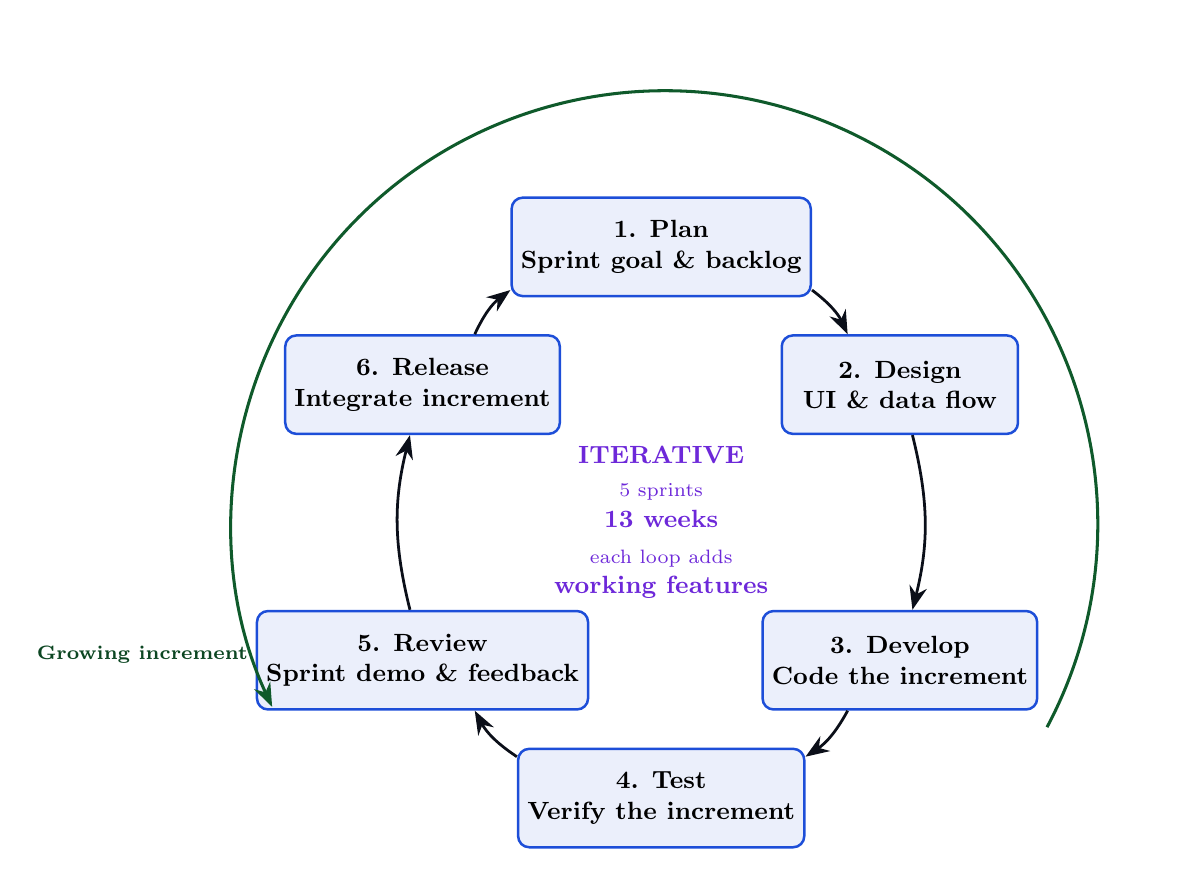
\begin{tikzpicture}[
  phase/.style={draw=appBlue, fill=appBlue!9, line width=0.9pt, rounded corners=4pt,
                minimum width=3.0cm, minimum height=1.25cm, align=center, font=\small\bfseries},
  phaselab/.style={font=\scriptsize, text=black!70, align=center},
  arc/.style={-{Stealth[length=3mm]}, line width=1pt, draw=appNavy}
]
% six phases on a circle
\node[phase] (p1) at (90:3.5cm)  {1. Plan\\{\phaselab Sprint goal \& backlog}};
\node[phase] (p2) at (30:3.5cm)  {2. Design\\{\phaselab UI \& data flow}};
\node[phase] (p3) at (-30:3.5cm) {3. Develop\\{\phaselab Code the increment}};
\node[phase] (p4) at (-90:3.5cm) {4. Test\\{\phaselab Verify the increment}};
\node[phase] (p5) at (-150:3.5cm){5. Review\\{\phaselab Sprint demo \& feedback}};
\node[phase] (p6) at (150:3.5cm) {6. Release\\{\phaselab Integrate increment}};

\draw[arc] (p1) to[bend left=14] (p2);
\draw[arc] (p2) to[bend left=14] (p3);
\draw[arc] (p3) to[bend left=14] (p4);
\draw[arc] (p4) to[bend left=14] (p5);
\draw[arc] (p5) to[bend left=14] (p6);
\draw[arc] (p6) to[bend left=14] (p1);

\node[align=center, font=\small\bfseries, text=appViolet] at (0,0)
     {ITERATIVE\\[1pt]\normalfont\scriptsize 5 sprints\\
      13 weeks\\[2pt]\normalfont\scriptsize each loop adds\\
      working features};

% outer growth arrow
\draw[-{Stealth[length=3mm]}, line width=1.1pt, draw=appGreen!70!black]
      (4.9,-2.6) arc[start angle=-28, end angle=205, radius=5.5cm]
      node[pos=0.98, above left, font=\scriptsize\bfseries, text=appGreen!55!black]
      {Growing increment};
\end{tikzpicture}
\caption{Agile iterative-incremental software development life cycle adopted for
StudyMate AI. Each pass through the six phases produces one working increment.}
\label{fig:sdlc}
\end{figure}

\section{Phase-wise Activities Mapped to This Project}

Table~\ref{tab:phases} maps each phase of the chosen life cycle to the activities actually performed and to the artefacts those activities produced.

\begin{table}[H]
\centering
\caption{Life-cycle phases and the concrete activities performed}
\label{tab:phases}
\small
\begin{tabularx}{\textwidth}{@{}p{2.9cm}X@{}}
\toprule
\rowcolor{tblhead} \textcolor{white}{\textbf{Phase}} &
\textcolor{white}{\textbf{Activities performed in this project}} \\
\midrule
1. Planning & Idea finalisation, feasibility check, team role allocation, backlog
  creation, sprint goal definition, schedule and risk identification. \\
2. Requirement Analysis & Elicitation of 18 functional and 12 non-functional
  requirements, user stories, use-case modelling, requirement traceability matrix. \\
3. Design & Three-tier architecture, DFD Levels 0--2, entity--relationship model,
  screen navigation graph, REST API contract, AsyncStorage key schema, dark-theme
  design system, UI mockups. \\
4. Implementation & Expo/TypeScript frontend (nine screens), Firebase
  authentication, AsyncStorage persistence, Node/Express backend, Gemini
  integration, Android build configuration. \\
5. Testing & Manual unit-level checks per function, integration testing of the
  app--backend link, emulator and physical-device testing, negative testing of AI
  validation, user-acceptance testing. \\
6. Deployment \& Review & Sprint demonstrations, defect fixing, Android APK build,
  documentation, final report, retrospective and future-work planning. \\
\bottomrule
\end{tabularx}
\end{table}

\section{Sprint Plan}

Table~\ref{tab:sprints} records the five development sprints, the goal of each and the working increment demonstrated at the end of each.

\begin{table}[H]
\centering
\caption{Sprint plan with goals and delivered increments}
\label{tab:sprints}
\small
\begin{tabularx}{\textwidth}{@{}p{1.5cm}p{2.5cm}Xp{3.1cm}@{}}
\toprule
\rowcolor{tblhead} \textcolor{white}{\textbf{Sprint}} &
\textcolor{white}{\textbf{Dates}} &
\textcolor{white}{\textbf{Goal}} &
\textcolor{white}{\textbf{Increment delivered}} \\
\midrule
Sprint 1 & 27 Jul -- 9 Aug 2026  & Project foundation and the authentication user
  interface & Navigable app shell; Welcome, Login and Register screens with the
  dark design system \\
Sprint 2 & 5 -- 18 Aug 2026      & Working authentication and the dashboard &
  Registration, login, password reset, sign-out, display name, route guard, Home
  dashboard \\
Sprint 3 & 15 -- 29 Aug 2026     & Personal data modules & Notes CRUD with search
  and the Study Planner, both isolated per user ID \\
Sprint 4 & 24 Aug -- 8 Sep 2026  & AI service layer & Express server with three
  Gemini endpoints, retry logic and quiz validation \\
Sprint 5 & 1 -- 14 Sep 2026      & AI user interfaces and integration & AI Chat,
  PDF Summary and Quiz screens connected end to end on the emulator \\
\bottomrule
\end{tabularx}
\end{table}

\noindent\textbf{Sprint cadence.} Each sprint consisted of: a planning meeting
(backlog selection and task split), daily 10-minute stand-ups, development, an
internal review with a test checklist, and a retrospective that fed corrections into
the next sprint's backlog.

\section{Project Schedule (Gantt Chart)}

The schedule in Figure~\ref{fig:gantt} spans the full project duration from
5 July 2026 to 30 September 2026. Analysis and design overlap intentionally with the
early sprints, which is characteristic of an iterative model.

\begin{landscape}
\begin{figure}[H]
\centering
\small
\begin{ganttchart}[
  hgrid,
  vgrid={*6{dotted,gray!45},{gray!80}},
  time slot format=isodate,
  x unit=0.175cm,
  y unit title=0.50cm,
  y unit chart=0.29cm,
  title label font=\tiny,
  bar label font=\tiny,
  group label font=\tiny\bfseries,
  milestone label font=\tiny\itshape,
  bar height=0.62,
  bar top shift=0.19,
  group height=0.42,
  group top shift=0.29,
  group left shift=0, group right shift=0,
  milestone/.append style={fill=appAmber, draw=appAmber},
  bar/.append style={fill=appBlue!70, draw=appBlue},
  group/.append style={fill=appViolet!70, draw=appViolet}
]{2026-07-05}{2026-09-30}
\gantttitle{July 2026}{27}\gantttitle{August 2026}{31}\gantttitle{September 2026}{30}\\
\gantttitle{W1}{7}\gantttitle{W2}{7}\gantttitle{W3}{7}\gantttitle{W4}{7}%
\gantttitle{W5}{7}\gantttitle{W6}{7}\gantttitle{W7}{7}\gantttitle{W8}{7}%
\gantttitle{W9}{7}\gantttitle{W10}{7}\gantttitle{W11}{7}\gantttitle{W12}{7}%
\gantttitle{W13}{4}\\

\ganttgroup{1. Inception \& Planning}{2026-07-05}{2026-07-11}\\
\ganttbar{Idea finalisation, team roles}{2026-07-05}{2026-07-08}\\
\ganttbar{Feasibility study}{2026-07-07}{2026-07-11}\\

\ganttgroup{2. Requirement Analysis}{2026-07-08}{2026-07-18}\\
\ganttbar{Gather functional \& non-functional req.}{2026-07-08}{2026-07-15}\\
\ganttbar{Use cases and user stories}{2026-07-12}{2026-07-18}\\
\ganttmilestone{M1 Requirements frozen}{2026-07-18}\\

\ganttgroup{3. System Design}{2026-07-15}{2026-07-26}\\
\ganttbar{Architecture and DFD design}{2026-07-15}{2026-07-21}\\
\ganttbar{UI/UX mockups, design system}{2026-07-18}{2026-07-25}\\
\ganttbar{Data schema and API contract}{2026-07-21}{2026-07-26}\\
\ganttmilestone{M2 Design approved}{2026-07-26}\\

\ganttgroup{4. Sprint 1 -- Foundation \& Auth UI}{2026-07-27}{2026-08-09}\\
\ganttbar{Expo setup, router, dark theme}{2026-07-27}{2026-08-02}\\
\ganttbar{Welcome / Login / Register screens}{2026-08-01}{2026-08-09}\\

\ganttgroup{5. Sprint 2 -- Firebase Auth \& Dashboard}{2026-08-05}{2026-08-18}\\
\ganttbar{Firebase Auth integration}{2026-08-05}{2026-08-12}\\
\ganttbar{Route guard, sign out, display name}{2026-08-09}{2026-08-16}\\
\ganttbar{Home dashboard and progress card}{2026-08-11}{2026-08-18}\\
\ganttmilestone{M3 Authentication working}{2026-08-18}\\

\ganttgroup{6. Sprint 3 -- Notes \& Planner}{2026-08-15}{2026-08-29}\\
\ganttbar{Notes CRUD and search}{2026-08-15}{2026-08-23}\\
\ganttbar{Study planner CRUD}{2026-08-18}{2026-08-27}\\
\ganttbar{Per-user storage partitioning}{2026-08-22}{2026-08-29}\\
\ganttmilestone{M4 Data modules complete}{2026-08-29}\\

\ganttgroup{7. Sprint 4 -- AI Backend}{2026-08-24}{2026-09-08}\\
\ganttbar{Express server and Gemini client}{2026-08-24}{2026-08-30}\\
\ganttbar{POST /chat streaming endpoint}{2026-08-28}{2026-09-03}\\
\ganttbar{POST /summarize-pdf (multer, base64)}{2026-08-31}{2026-09-06}\\
\ganttbar{POST /generate-quiz and validation}{2026-09-02}{2026-09-08}\\
\ganttmilestone{M5 AI backend live}{2026-09-08}\\

\ganttgroup{8. Sprint 5 -- AI Screens \& Integration}{2026-09-01}{2026-09-14}\\
\ganttbar{Chat / PDF / Quiz screens}{2026-09-01}{2026-09-09}\\
\ganttbar{End-to-end integration, emulator net.}{2026-09-07}{2026-09-14}\\
\ganttmilestone{M6 Feature complete}{2026-09-14}\\

\ganttgroup{9. Testing \& Quality Assurance}{2026-09-10}{2026-09-22}\\
\ganttbar{Manual and device testing}{2026-09-10}{2026-09-18}\\
\ganttbar{Defect fixing and regression}{2026-09-14}{2026-09-22}\\
\ganttmilestone{M7 Testing complete}{2026-09-22}\\

\ganttgroup{10. Release \& Documentation}{2026-09-20}{2026-09-30}\\
\ganttbar{Android build (prebuild / APK)}{2026-09-20}{2026-09-26}\\
\ganttbar{Report writing and documentation}{2026-09-22}{2026-09-30}\\
\ganttmilestone{M8 Final submission}{2026-09-30}
\end{ganttchart}
\caption{Project Gantt chart, 5 July 2026 -- 30 September 2026. Vertical grid lines
mark week boundaries; amber diamonds are milestones M1--M8.}
\label{fig:gantt}
\end{figure}
\end{landscape}

\section{Milestones}

Table~\ref{tab:milestones} lists the eight project milestones with the date each was reached and the evidence used to accept it.

\begin{table}[H]
\centering
\caption{Project milestones and acceptance evidence}
\label{tab:milestones}
\small
\begin{tabularx}{\textwidth}{@{}p{1.1cm}p{2.5cm}p{5.2cm}X@{}}
\toprule
\rowcolor{tblhead} \textcolor{white}{\textbf{ID}} &
\textcolor{white}{\textbf{Date}} &
\textcolor{white}{\textbf{Milestone}} &
\textcolor{white}{\textbf{Acceptance evidence}} \\
\midrule
M1 & 18 Jul 2026 & Requirements frozen        & Signed-off requirement list and use-case diagram \\
M2 & 26 Jul 2026 & Design approved            & Architecture, DFD Levels 0--2 and UI mockups reviewed \\
M3 & 18 Aug 2026 & Authentication working     & Registration, login, reset and guard demonstrated on the emulator \\
M4 & 29 Aug 2026 & Data modules complete      & Notes and planner persist correctly for two separate accounts \\
M5 &  8 Sep 2026 & AI backend live            & All three endpoints return valid responses via \texttt{curl} \\
M6 & 14 Sep 2026 & Feature complete           & Every screen reachable and functional end to end \\
M7 & 22 Sep 2026 & Testing complete           & All test cases executed, critical defects closed \\
M8 & 30 Sep 2026 & Final submission           & Android build plus this report submitted \\
\bottomrule
\end{tabularx}
\end{table}

\section{Work Breakdown Structure}

The work breakdown structure in Figure~\ref{fig:wbs} decomposes the project into
seven level-2 work packages, each broken down into its level-3 sub-packages. The
package numbers are reused unchanged in the task allocation matrix of
Chapter~\ref{ch:pm}, so every task performed in the project can be traced to exactly
one package and one responsible member.

\begin{landscape}
\begin{figure}[H]
\centering
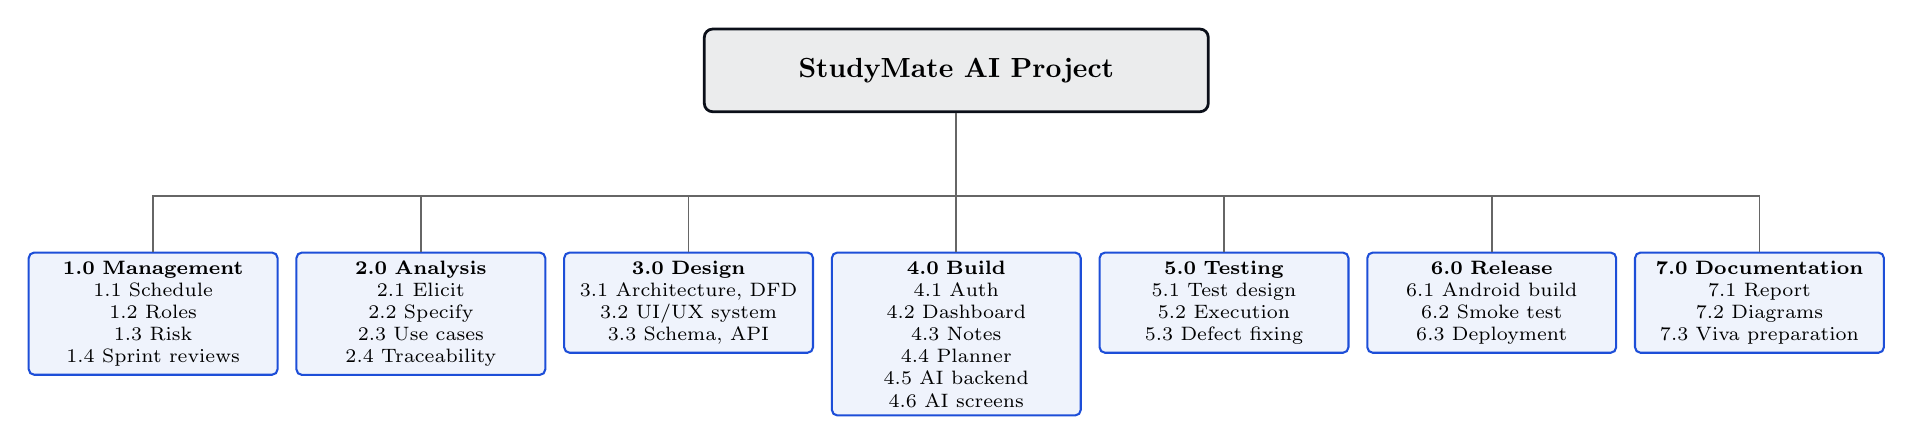
\begin{tikzpicture}[
  lvl1/.style={draw=appNavy, fill=appNavy!8, line width=1pt, rounded corners=3pt,
               minimum width=6.4cm, minimum height=1.05cm, align=center,
               font=\normalsize\bfseries},
  lvl2/.style={draw=appBlue, fill=appBlue!7, line width=0.75pt, rounded corners=2pt,
               align=center, font=\scriptsize, inner sep=3pt, text width=2.95cm,
               anchor=north},
  edge/.style={draw=black!60, line width=0.6pt}
]
\node[lvl1] (root) at (0,0) {StudyMate AI Project};

\node[lvl2] (p1) at (-10.20,-2.30) {\textbf{1.0 Management}\\ 1.1 Schedule\\ 1.2 Roles\\ 1.3 Risk\\ 1.4 Sprint reviews};
\node[lvl2] (p2) at (-6.80,-2.30)  {\textbf{2.0 Analysis}\\ 2.1 Elicit\\ 2.2 Specify\\ 2.3 Use cases\\ 2.4 Traceability};
\node[lvl2] (p3) at (-3.40,-2.30)  {\textbf{3.0 Design}\\ 3.1 Architecture, DFD\\ 3.2 UI/UX system\\ 3.3 Schema, API};
\node[lvl2] (p4) at (0.00,-2.30)   {\textbf{4.0 Build}\\ 4.1 Auth\\ 4.2 Dashboard\\ 4.3 Notes\\ 4.4 Planner\\ 4.5 AI backend\\ 4.6 AI screens};
\node[lvl2] (p5) at (3.40,-2.30)   {\textbf{5.0 Testing}\\ 5.1 Test design\\ 5.2 Execution\\ 5.3 Defect fixing};
\node[lvl2] (p6) at (6.80,-2.30)   {\textbf{6.0 Release}\\ 6.1 Android build\\ 6.2 Smoke test\\ 6.3 Deployment};
\node[lvl2] (p7) at (10.20,-2.30)  {\textbf{7.0 Documentation}\\ 7.1 Report\\ 7.2 Diagrams\\ 7.3 Viva preparation};

\draw[edge] (root.south) -- ++(0,-1.05) -| (p1.north);
\draw[edge] (root.south) -- ++(0,-1.05) -| (p2.north);
\draw[edge] (root.south) -- ++(0,-1.05) -| (p3.north);
\draw[edge] (root.south) -- (p4.north);
\draw[edge] (root.south) -- ++(0,-1.05) -| (p5.north);
\draw[edge] (root.south) -- ++(0,-1.05) -| (p6.north);
\draw[edge] (root.south) -- ++(0,-1.05) -| (p7.north);
\end{tikzpicture}
\caption{Work breakdown structure of the StudyMate AI project (levels 1--3). The
level-2 and level-3 package numbers are the identifiers used in the task allocation
matrix, Table~\ref{tab:alloc}.}
\label{fig:wbs}
\end{figure}
\end{landscape}

% =====================================================================
\chapter{Requirement Analysis and Specification}\label{ch:req}
% =====================================================================

\section{Functional Requirements}

Table~\ref{tab:fr} lists the twenty-two functional requirements (FR-01 to FR-22) elicited from the project brief. Every one of them is carried forward through design, implementation and testing in the traceability matrix of Table~\ref{tab:rtm}.

\begin{longtable}{@{}p{1.5cm}p{4.6cm}p{6.3cm}p{2.1cm}@{}}
\caption{Functional requirements} \label{tab:fr} \\
\toprule
\rowcolor{tblhead} \textcolor{white}{\textbf{ID}} &
\textcolor{white}{\textbf{Requirement}} &
\textcolor{white}{\textbf{Description}} &
\textcolor{white}{\textbf{Priority}} \\
\midrule
\endfirsthead
\caption[]{Functional requirements (continued)} \\
\toprule
\rowcolor{tblhead} \textcolor{white}{\textbf{ID}} &
\textcolor{white}{\textbf{Requirement}} &
\textcolor{white}{\textbf{Description}} &
\textcolor{white}{\textbf{Priority}} \\
\midrule
\endhead
FR-01 & User registration & The system shall allow a new user to register with full
   name, e-mail and password, and shall store the name as the account display name. & High \\
FR-02 & User login & The system shall authenticate a registered user with e-mail and
   password. & High \\
FR-03 & Password reset & The system shall send a password-reset e-mail on request. & High \\
FR-04 & Logout & The system shall sign the user out after confirmation and return to
   the login screen. & High \\
FR-05 & Screen protection & The system shall prevent an unauthenticated user from
   reaching the dashboard. & High \\
FR-06 & Display user identity & The system shall greet the user by display name and
   show an avatar built from the name initials. & Medium \\
FR-07 & Create note & The system shall let the user create a note with a title and
   body, requiring both to be non-empty. & High \\
FR-08 & Edit note & The system shall let the user modify an existing note in place,
   preserving list order. & High \\
FR-09 & Delete note & The system shall delete a note only after explicit
   confirmation. & High \\
FR-10 & Search notes & The system shall filter notes by a case-insensitive keyword
   matched against title and body. & Medium \\
FR-11 & Per-user note isolation & The system shall store notes under a key scoped to
   the authenticated user ID. & High \\
FR-12 & Add study session & The system shall let the user add a session with subject,
   date and duration, validating all three fields. & High \\
FR-13 & Complete / undo session & The system shall toggle a session's completion
   state and persist the change. & High \\
FR-14 & Delete study session & The system shall delete a session after confirmation. & Medium \\
FR-15 & Progress calculation & The system shall compute completed, remaining and
   percentage values and display them on the planner and the dashboard. & High \\
FR-16 & Dashboard refresh & The dashboard shall reload session data whenever the
   screen regains focus. & Medium \\
FR-17 & AI chat & The system shall send the user's question to the AI service and
   display the answer as a chat bubble. & High \\
FR-18 & PDF summarisation & The system shall accept a PDF (maximum 10\,MB) and return
   a structured summary. & High \\
FR-19 & Quiz generation & The system shall generate a multiple-choice quiz for a
   given topic, question count (5/10/15) and difficulty (easy/medium/hard). & High \\
FR-20 & Quiz interaction & The system shall mark answers immediately, reveal an
   explanation, track the score and show a final accuracy percentage. & High \\
FR-21 & AI output validation & The backend shall validate model output and reject
   malformed quizzes before they reach the client. & High \\
FR-22 & AI key protection & The Gemini API key shall reside only on the backend. & High \\
\bottomrule
\end{longtable}

\section{Non-Functional Requirements}

Table~\ref{tab:nfr} lists the twelve non-functional requirements, which constrain the quality of the system rather than its behaviour.

\begin{table}[H]
\centering
\caption{Non-functional requirements}
\label{tab:nfr}
\small
\begin{tabularx}{\textwidth}{@{}p{1.5cm}p{2.7cm}X@{}}
\toprule
\rowcolor{tblhead} \textcolor{white}{\textbf{ID}} &
\textcolor{white}{\textbf{Category}} &
\textcolor{white}{\textbf{Requirement}} \\
\midrule
NFR-01 & Usability       & A consistent dark theme, a single thumb-reachable primary
   action per screen and a back affordance on every feature screen. \\
NFR-02 & Performance     & Local screens (notes, planner, dashboard) must render
   without network latency; AI responses should begin within a few seconds. \\
NFR-03 & Reliability     & AI calls shall retry with exponential backoff on rate-limit
   and server errors; every failure path shall show a user-friendly message. \\
NFR-04 & Security        & Passwords are never stored by the application; the AI key
   is server-side only; user data is isolated by user ID. \\
NFR-05 & Privacy         & Uploaded PDFs are held in server memory only and are never
   written to disk. \\
NFR-06 & Portability     & One codebase shall build for Android, iOS and web. \\
NFR-07 & Maintainability & Strict TypeScript, one shared authentication instance, one
   writer function per storage collection, and centralised backend configuration. \\
NFR-08 & Compatibility   & Android 8 and above; edge-to-edge display support. \\
NFR-09 & Availability    & Local data modules remain fully usable when the AI backend
   is offline. \\
NFR-10 & Accessibility   & Minimum readable contrast on a dark background; labels on
   every input field. \\
NFR-11 & Scalability     & The backend is stateless, so additional AI endpoints or
   instances can be added without data migration. \\
NFR-12 & Documentation   & Every module shall be traceable from requirement to source
   line and to test case. \\
\bottomrule
\end{tabularx}
\end{table}

\section{User Stories}

Table~\ref{tab:stories} records the eight user stories written during requirement analysis together with the acceptance criteria against which each was later tested.

\begin{table}[H]
\centering
\caption{Representative user stories with acceptance criteria}
\label{tab:stories}
\small
\begin{tabularx}{\textwidth}{@{}p{1.1cm}Xp{4.6cm}@{}}
\toprule
\rowcolor{tblhead} \textcolor{white}{\textbf{ID}} &
\textcolor{white}{\textbf{User story}} &
\textcolor{white}{\textbf{Acceptance criteria}} \\
\midrule
US-01 & As a new student I want to create an account with my name so that the app
   can greet me personally. & Account is created; the name appears in the dashboard
   greeting and as initials in the avatar. \\
US-02 & As a student I want to reset a forgotten password so that I can regain
   access. & A reset e-mail arrives; after changing the password the old one no
   longer works. \\
US-03 & As a student I want my notes to be private so that another account on the
   same phone cannot read them. & Signing in with a different account shows an empty
   note list. \\
US-04 & As a student I want to search my notes so that I can revise quickly. &
   Typing a keyword filters the list by title or body; a clear message appears when
   nothing matches. \\
US-05 & As a student I want to mark a session done so that my progress updates. &
   The card changes state, the planner percentage rises, and the dashboard updates
   when I return to it. \\
US-06 & As a student I want to upload a lecture PDF so that I get revision notes. &
   A summary with headings and bullet points is displayed. \\
US-07 & As a student I want a quiz on my topic so that I can test myself. & The
   requested number of questions appears; answers are marked; explanations and a
   final score are shown. \\
US-08 & As a student I want a clear message when the AI is unavailable so that I am
   not confused by a frozen screen. & A friendly error bubble or alert is shown and
   the input becomes usable again. \\
\bottomrule
\end{tabularx}
\end{table}

\section{Use-Case Model}

Figure~\ref{fig:usecase} presents the use-case diagram of the system. The student is the only human actor; the Gemini service appears as a secondary actor because it is invoked through the backend rather than directly by the application.

\begin{figure}[H]
\centering
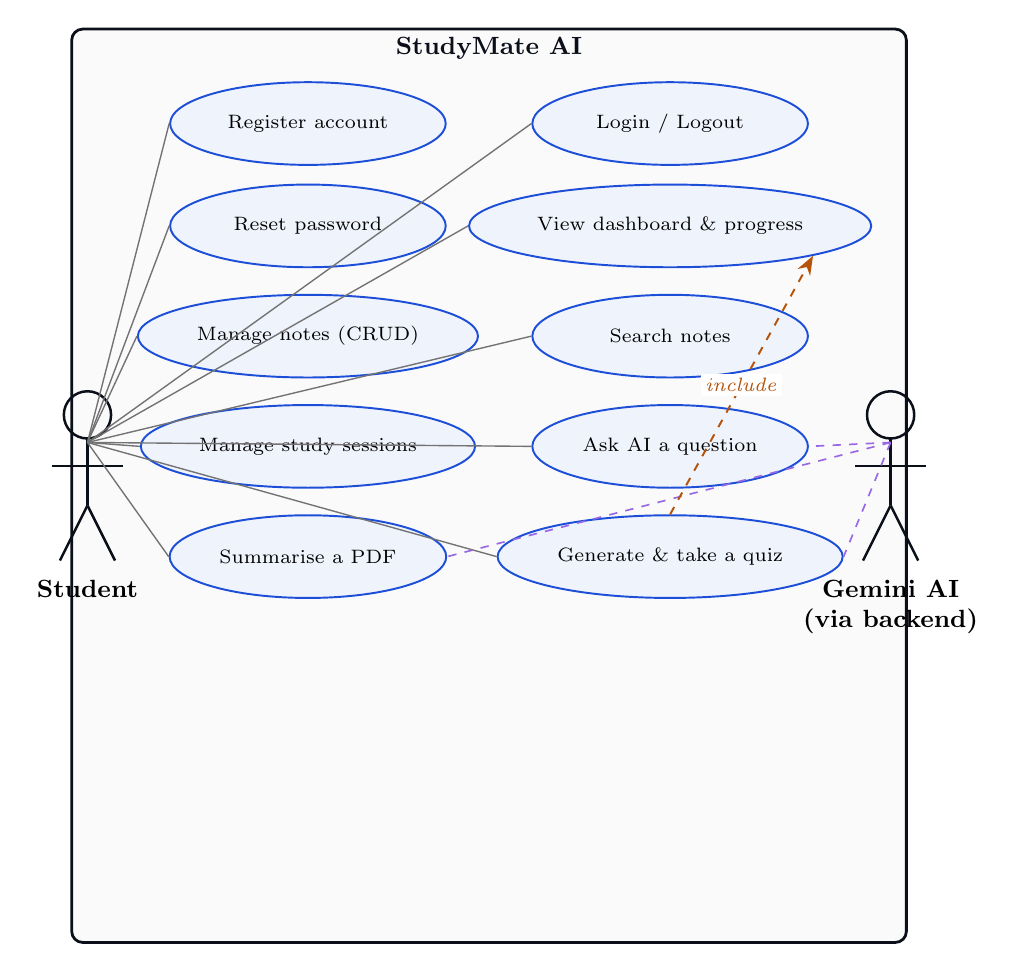
\begin{tikzpicture}[
  actor/.style={font=\small\bfseries},
  stick/.style={line width=0.9pt, draw=appNavy}
]
% system boundary
\node[draw=appNavy, line width=1pt, rounded corners=4pt, fill=appNavy!2,
      minimum width=10.6cm, minimum height=11.6cm, inner sep=8pt] (sys) at (5.3,0) {};
\node[font=\small\bfseries, text=appNavy] at (5.3,5.55) {StudyMate AI};

% student actor (left)
\begin{scope}[shift={(0.2,-0.2)}]
  \draw[stick] (0,1.1) circle (0.30);
  \draw[stick] (0,0.8) -- (0,-0.05);
  \draw[stick] (-0.45,0.45) -- (0.45,0.45);
  \draw[stick] (0,-0.05) -- (-0.35,-0.75);
  \draw[stick] (0,-0.05) -- (0.35,-0.75);
  \node[actor, below=0.12cm] at (0,-0.75) {Student};
\end{scope}

% gemini actor (right)
\begin{scope}[shift={(10.4,-0.2)}]
  \draw[stick] (0,1.1) circle (0.30);
  \draw[stick] (0,0.8) -- (0,-0.05);
  \draw[stick] (-0.45,0.45) -- (0.45,0.45);
  \draw[stick] (0,-0.05) -- (-0.35,-0.75);
  \draw[stick] (0,-0.05) -- (0.35,-0.75);
  \node[actor, below=0.12cm, align=center] at (0,-0.75) {Gemini AI\\(via backend)};
\end{scope}

% use cases
\node[uc] (u1) at (3.0, 4.6) {Register account};
\node[uc] (u2) at (7.6, 4.6) {Login / Logout};
\node[uc] (u3) at (3.0, 3.3) {Reset password};
\node[uc] (u4) at (7.6, 3.3) {View dashboard \& progress};
\node[uc] (u5) at (3.0, 1.9) {Manage notes (CRUD)};
\node[uc] (u6) at (7.6, 1.9) {Search notes};
\node[uc] (u7) at (3.0, 0.5) {Manage study sessions};
\node[uc] (u8) at (7.6, 0.5) {Ask AI a question};
\node[uc] (u9) at (3.0,-0.9) {Summarise a PDF};
\node[uc] (u10) at (7.6,-0.9) {Generate \& take a quiz};

% student associations
\foreach \u in {u1,u2,u3,u4,u5,u6,u7,u8,u9,u10}
  \draw[draw=black!55, line width=0.5pt] (0.2,0.55) -- (\u.west);

% gemini associations
\foreach \u in {u8,u9,u10}
  \draw[draw=appViolet!70, line width=0.6pt, dashed] (10.4,0.55) -- (\u.east);

% include relationship
\draw[-{Stealth[length=2.4mm]}, draw=appAmber, line width=0.7pt, dashed]
   (u10.north) -- node[flab, midway] {\textcolor{appAmber}{\scriptsize\textit{include}}} (u4.south east);
\end{tikzpicture}
\caption{Use-case diagram of StudyMate AI. Solid lines are student interactions;
dashed violet lines are AI-service dependencies; the amber dashed arrow is an
\emph{include} relationship (taking a quiz includes viewing the resulting progress
feedback).}
\label{fig:usecase}
\end{figure}

\subsection{Use-Case Descriptions}

Table~\ref{tab:usecasedesc} expands the two most important use cases into the full description template used in the software requirement specification.

\begin{table}[H]
\centering
\caption{Detailed description of two principal use cases}
\label{tab:usecasedesc}
\small
\begin{tabularx}{\textwidth}{@{}>{\bfseries}p{3.0cm}X@{}}
\toprule
\multicolumn{2}{@{}l@{}}{\textbf{UC-01: Log in to the application}} \\
\midrule
Actor          & Student (authenticated) \\
Precondition   & An account already exists; the application is at the login screen. \\
Main flow      & 1. The student enters e-mail and password. 2. The student taps
                 \emph{Login}. 3. The system validates that both fields are filled.
                 4. The system sends the credentials to Firebase Authentication.
                 5. Firebase confirms the identity and returns a user object.
                 6. The system navigates to the Home Dashboard. 7. The dashboard
                 loads the display name and the user's study sessions. \\
Alternate flow & 4a. Invalid credentials: Firebase returns an error code; the system
                 displays a specific message (unknown account, wrong password,
                 invalid e-mail) and returns focus to the form. \\
Postcondition  & The student is authenticated and the dashboard is displayed. \\
\midrule
\multicolumn{2}{@{}l@{}}{\textbf{UC-02: Generate and take an AI quiz}} \\
\midrule
Actor          & Student; Gemini AI (secondary) \\
Precondition   & The AI backend is running and reachable. \\
Main flow      & 1. The student enters a topic. 2. The student selects a question
                 count (5, 10 or 15) and a difficulty. 3. The student taps
                 \emph{Generate Quiz}. 4. The client posts the parameters to the
                 backend. 5. The backend clamps the count, builds a strict prompt and
                 calls Gemini. 6. The backend strips code fences, parses the JSON and
                 validates every question. 7. The validated quiz is returned.
                 8. The student answers each question and receives immediate marking
                 and an explanation. 9. After the last question the final score and
                 accuracy are shown. \\
Alternate flow & 6a. Malformed JSON: the backend responds with an error and the client
                 shows a retry alert. 4a. Backend unreachable: a connection alert is
                 shown and the setup form remains available. \\
Postcondition  & The attempt is displayed in memory; it is not persisted after the
                 screen is left. \\
\bottomrule
\end{tabularx}
\end{table}

\section{Requirement Traceability Matrix}

Table~\ref{tab:rtm} traces every requirement to its design artefact, implementation
source location and test case, satisfying the course requirement for end-to-end
traceability.

\begin{landscape}
\begin{longtable}{@{}p{1.3cm}p{3.5cm}p{3.4cm}p{5.4cm}p{2.0cm}p{1.6cm}@{}}
\caption{Requirement traceability matrix} \label{tab:rtm} \\
\toprule
\rowcolor{tblhead} \textcolor{white}{\textbf{Req.}} &
\textcolor{white}{\textbf{Design artefact}} &
\textcolor{white}{\textbf{Module}} &
\textcolor{white}{\textbf{Source location}} &
\textcolor{white}{\textbf{Test case}} &
\textcolor{white}{\textbf{Status}} \\
\midrule
\endfirsthead
\toprule
\rowcolor{tblhead} \textcolor{white}{\textbf{Req.}} &
\textcolor{white}{\textbf{Design artefact}} &
\textcolor{white}{\textbf{Module}} &
\textcolor{white}{\textbf{Source location}} &
\textcolor{white}{\textbf{Test case}} &
\textcolor{white}{\textbf{Status}} \\
\midrule
\endhead
FR-01 & Use case UC-01; DFD 1.0 & Authentication & \fp{app/register.tsx} lines 54--116 & TC-01 & \yes \\
FR-02 & Use case UC-01; DFD 1.0 & Authentication & \fp{app/login.tsx} lines 50--84 & TC-02 & \yes \\
FR-03 & DFD 1.0 & Authentication & \fp{app/login.tsx} lines 87--113 & TC-03 & \yes \\
FR-04 & Navigation flow & Authentication & \fp{app/(tabs)/index.tsx} lines 121--153 & TC-04 & \yes \\
FR-05 & Auth flowchart; DFD 1.0 & Navigation guard & \fp{app/_layout.tsx} lines 41--79 & TC-05 & Partial \\
FR-06 & Dashboard design & Dashboard & \fp{app/(tabs)/index.tsx} lines 63--72, 189--205 & TC-06 & \yes \\
FR-07 & DFD 2.0; ER model & Notes & \fp{app/notes.tsx} lines 120--171 & TC-07 & \yes \\
FR-08 & DFD 2.0 & Notes & \fp{app/notes.tsx} lines 137--146, 173--178 & TC-08 & \yes \\
FR-09 & DFD 2.0 & Notes & \fp{app/notes.tsx} lines 180--202 & TC-09 & \yes \\
FR-10 & DFD 2.0 & Notes & \fp{app/notes.tsx} lines 211--218 & TC-10 & \yes \\
FR-11 & Data design; ER model & Notes storage & \fp{app/notes.tsx} lines 90, 109 & TC-11 & \yes \\
FR-12 & DFD 3.0; ER model & Planner & \fp{app/study-planner.tsx} lines 141--197 & TC-12 & \yes \\
FR-13 & DFD 3.0 & Planner & \fp{app/study-planner.tsx} lines 203--223 & TC-13 & \yes \\
FR-14 & DFD 3.0 & Planner & \fp{app/study-planner.tsx} lines 229--260 & TC-14 & \yes \\
FR-15 & DFD 5.0 & Progress engine & \fp{app/study-planner.tsx} 266--275; \fp{app/(tabs)/index.tsx} 170--184 & TC-15 & \yes \\
FR-16 & Sequence of focus events & Dashboard & \fp{app/(tabs)/index.tsx} lines 108--116 & TC-16 & \yes \\
FR-17 & DFD Level 2 (5.1) & AI Chat & \fp{app/ai-chat.tsx} 41--126; \fp{backend/server.js} 114--238 & TC-17 & \yes \\
FR-18 & DFD Level 2 (5.2) & PDF Summary & \fp{app/pdf-summary.tsx} 34--121; \fp{backend/server.js} 243--317 & TC-18 & \yes \\
FR-19 & DFD Level 2 (5.3) & AI Quiz & \fp{app/quiz.tsx} 49--91; \fp{backend/server.js} 322--519 & TC-19 & \yes \\
FR-20 & Quiz state machine & AI Quiz & \fp{app/quiz.tsx} lines 97--135 & TC-20 & \yes \\
FR-21 & Backend validation & AI Quiz & \fp{backend/server.js} lines 442--505 & TC-21 & \yes \\
FR-22 & Security design & Backend & \fp{backend/server.js} lines 31--41; \fp{.gitignore} lines 2--4 & TC-22 & \yes \\
\bottomrule
\end{longtable}
\end{landscape}

% =====================================================================
\chapter{System Design}\label{ch:design}
% =====================================================================

\section{System Architecture}

StudyMate AI uses a three-tier architecture. The presentation tier is the Expo
application; the identity tier is Firebase Authentication; the AI service tier is a
self-hosted Express server that mediates all access to Google Gemini. Content data
lives in a fourth, device-local tier (AsyncStorage). Figure~\ref{fig:arch} shows
the four tiers and the direction of every call between them.

\begin{figure}[H]
\centering
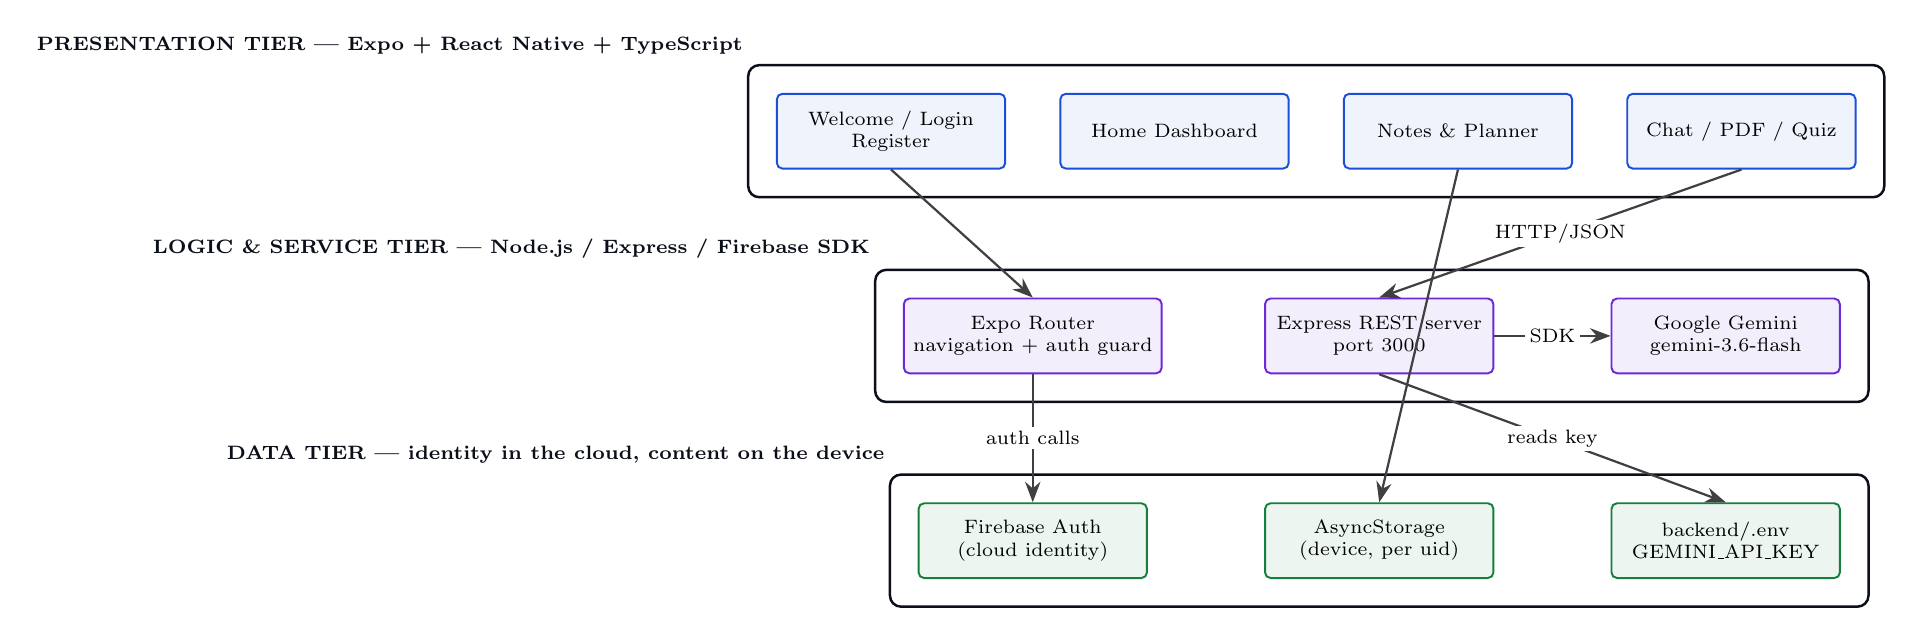
\begin{tikzpicture}[
  tier/.style={draw=appNavy, line width=0.9pt, rounded corners=4pt, fill=white,
               inner sep=7pt},
  tiertitle/.style={font=\scriptsize\bfseries, text=appNavy},
  comp/.style={draw=appBlue, fill=appBlue!7, line width=0.7pt, rounded corners=2pt,
               minimum width=2.9cm, minimum height=0.95cm, align=center, font=\scriptsize},
  svc/.style={draw=appViolet, fill=appViolet!8, line width=0.7pt, rounded corners=2pt,
               minimum width=2.9cm, minimum height=0.95cm, align=center, font=\scriptsize},
  store/.style={draw=appGreen, fill=appGreen!8, line width=0.7pt, rounded corners=2pt,
               minimum width=2.9cm, minimum height=0.95cm, align=center, font=\scriptsize},
  arr/.style={-{Stealth[length=2.6mm]}, line width=0.8pt, draw=black!75},
  lbl/.style={font=\scriptsize, fill=white, inner sep=1.5pt}
]
% presentation tier
\node[comp] (welcome) at (0,0)     {Welcome / Login\\Register};
\node[comp] (dash)    at (3.6,0)   {Home Dashboard};
\node[comp] (notes)   at (7.2,0)   {Notes \& Planner};
\node[comp] (ai)      at (10.8,0)  {Chat / PDF / Quiz};
\begin{scope}[on background layer]
\node[tier, fit=(welcome)(dash)(notes)(ai), inner sep=10pt] (t1) {};
\end{scope}
\node[tiertitle, above left=0pt and -2pt of t1.north west] {PRESENTATION TIER --- Expo + React Native + TypeScript};

% service tier
\node[svc] (router) at (1.8,-2.6) {Expo Router\\navigation + auth guard};
\node[svc] (express) at (6.2,-2.6) {Express REST server\\port 3000};
\node[svc] (gemini) at (10.6,-2.6) {Google Gemini\\gemini-3.6-flash};
\begin{scope}[on background layer]
\node[tier, fit=(router)(express)(gemini), inner sep=10pt] (t2) {};
\end{scope}
\node[tiertitle, above left=0pt and -2pt of t2.north west] {LOGIC \& SERVICE TIER --- Node.js / Express / Firebase SDK};

% data tier
\node[store] (fb)  at (1.8,-5.2) {Firebase Auth\\(cloud identity)};
\node[store] (as)  at (6.2,-5.2) {AsyncStorage\\(device, per uid)};
\node[store] (env) at (10.6,-5.2) {backend/.env\\GEMINI\_API\_KEY};
\begin{scope}[on background layer]
\node[tier, fit=(fb)(as)(env), inner sep=10pt] (t3) {};
\end{scope}
\node[tiertitle, above left=0pt and -2pt of t3.north west] {DATA TIER --- identity in the cloud, content on the device};

% arrows
\draw[arr] (welcome.south) -- (router.north);
\draw[arr] (ai.south) -- node[lbl, midway] {HTTP/JSON} (express.north);
\draw[arr] (notes.south) -- (as.north);
\draw[arr] (express.east) -- node[lbl, midway] {SDK} (gemini.west);
\draw[arr] (router.south) -- node[lbl, midway] {auth calls} (fb.north);
\draw[arr] (express.south) -- node[lbl, midway] {reads key} (env.north);
\end{tikzpicture}
\caption{Three-tier system architecture of StudyMate AI.}
\label{fig:arch}
\end{figure}

\section{Data Flow Diagram --- Level 0 (Context Diagram)}

The context diagram in Figure~\ref{fig:dfd0} defines the system boundary and its
external entities: the
student, Firebase Authentication and the Gemini AI service.

\begin{figure}[H]
\centering
\begin{tikzpicture}
\node[dfdentity, minimum width=2.7cm, minimum height=1.6cm] (stu) at (0,0) {STUDENT};
\node[draw=appBlue, fill=appBlue!8, line width=1.2pt, circle, minimum size=3.9cm,
      align=center, font=\small\bfseries] (sys) at (6.6,0) {0\\[2pt]\normalfont\small StudyMate AI\\System};
\node[dfdext] (fb) at (12.6,1.7)  {FIREBASE\\AUTHENTICATION};
\node[dfdext] (ai) at (12.6,-1.7) {GEMINI AI\\(via Express)};

\draw[flow] (stu.north east) -- node[flab, above, sloped] {credentials, notes, sessions,} node[flab, below, sloped] {questions, PDF, quiz topic} (sys.west |- 0.55);
\draw[rflow] (sys.west |- -0.55) -- node[flab, below, sloped] {identity, lists, progress, answers, summaries, quizzes} (stu.south east);

\draw[flow] (sys.north east) -- node[flab, above, sloped] {register / login / reset} (fb.west);
\draw[rflow] (fb.west |- 1.25) -- node[flab, below, sloped] {uid, displayName} (sys.north east |- 1.25);

\draw[flow] (sys.south east) -- node[flab, below, sloped] {prompt, PDF bytes, topic} (ai.west);
\draw[rflow] (ai.west |- -1.25) -- node[flab, above, sloped] {answer, summary, quiz JSON} (sys.south east |- -1.25);
\end{tikzpicture}
\caption{DFD Level 0 (context diagram). Green arrows are responses returning to the
student or the system.}
\label{fig:dfd0}
\end{figure}

\section{Data Flow Diagram --- Level 1}

Level 1, shown in Figure~\ref{fig:dfd1}, decomposes the system into five processes
and three data stores, using an
adapted Gane--Sarson notation: squares are external entities, rounded rectangles are
processes, and split rectangles are data stores.

\begin{figure}[H]
\centering
\begin{tikzpicture}
\node[dfdentity, minimum width=2.3cm, minimum height=2.2cm] (stu) at (0.0,4.4) {STUDENT};

\node[dfdproc] (p1) at (5.9,8.4) {\textbf{1.0}\\Manage Authentication};
\node[dfdproc] (p2) at (5.9,6.3) {\textbf{2.0}\\Manage Notes};
\node[dfdproc] (p3) at (5.9,4.2) {\textbf{3.0}\\Manage Study Plan};
\node[dfdproc] (p4) at (5.9,2.1) {\textbf{4.0}\\Present Dashboard\\and Progress};
\node[dfdproc] (p5) at (5.9,0.0) {\textbf{5.0}\\Generate AI Content};

\node[dfdstore, minimum width=4.0cm] (d1) at (12.3,8.4) {\textbf{D1} \nodepart{two} Firebase Accounts};
\node[dfdstore, minimum width=4.0cm] (d2) at (12.3,6.3) {\textbf{D2} \nodepart{two} Notes Store};
\node[dfdstore, minimum width=4.0cm] (d3) at (12.3,4.2) {\textbf{D3} \nodepart{two} Session Store};
\node[dfdext, minimum width=4.0cm]  (gem) at (12.3,0.0) {GEMINI AI};

% student <-> processes
\draw[flow] (stu.north east) -- node[flab, midway, above, sloped] {credentials} (p1.west);
\draw[flow] (stu.east |- 5.6) -- node[flab, midway, above] {note title, body} (p2.west);
\draw[flow] (stu.east) -- node[flab, midway, above] {subject, date, duration} (p3.west);
\draw[flow] (stu.east |- 2.9) -- node[flab, midway, below] {view request} (p4.west);
\draw[flow] (stu.south east) -- node[flab, midway, below, sloped] {question / PDF / topic} (p5.west);

\draw[rflow] (p1.west |- 8.0) -- node[flab, midway, below] {auth result, name} (stu.north east |- 8.0);
\draw[rflow] (p2.west |- 5.9) -- node[flab, midway, below] {note list} (stu.east |- 5.9);
\draw[rflow] (p3.west |- 3.8) -- node[flab, midway, below] {session list} (stu.east |- 3.8);
\draw[rflow] (p4.west |- 2.5) -- node[flab, midway, above] {progress, statistics} (stu.east |- 2.5);
\draw[rflow] (p5.west |- -0.4) -- node[flab, midway, above, sloped] {answer / summary / quiz} (stu.south east |- -0.4);

% processes <-> stores
\draw[flow] (p1.east) -- node[flab, midway, above] {write user} (d1.west);
\draw[rflow] (d1.west |- 8.05) -- node[flab, midway, below] {uid, displayName} (p1.east |- 8.05);

\draw[flow] (p2.east) -- node[flab, midway, above] {notes JSON} (d2.west);
\draw[rflow] (d2.west |- 5.95) -- node[flab, midway, below] {notes JSON} (p2.east |- 5.95);

\draw[flow] (p3.east) -- node[flab, midway, above] {sessions JSON} (d3.west);
\draw[rflow] (d3.west |- 3.85) -- node[flab, midway, below] {sessions JSON} (p3.east |- 3.85);

% dashboard reads both stores (routed outside)
\draw[rflow] (d2.east) -- ++(0.75,0) |- node[flab, pos=0.78, above] {notes count} (p4.east |- 2.35);
\draw[rflow] (d3.east) -- ++(0.45,0) |- node[flab, pos=0.78, below] {sessions} (p4.east |- 1.85);

% AI
\draw[flow] (p5.east) -- node[flab, midway, above] {prompt, PDF} (gem.west);
\draw[rflow] (gem.west |- -0.35) -- node[flab, midway, below] {model output} (p5.east |- -0.35);
\end{tikzpicture}
\caption{DFD Level 1. Note that process 5.0 has \emph{no} data store: AI output is
consumed immediately and is never persisted, which is an intentional design decision
documented as limitation L-2.}
\label{fig:dfd1}
\end{figure}

\section{Data Flow Diagram --- Level 2 (AI Subsystem)}

Process 5.0 is decomposed in Figure~\ref{fig:dfd2} to show the Express server
boundary and the three AI sub-processes.

\begin{figure}[H]
\centering
\begin{tikzpicture}
\node[dfdentity, minimum width=2.2cm, minimum height=2.0cm] (stu) at (-0.4,2.2) {STUDENT};

\node[dfdproc, minimum width=4.0cm] (c1) at (5.0,4.4) {\textbf{5.1}\\AI Chat Handler};
\node[dfdproc, minimum width=4.0cm] (c2) at (5.0,2.2) {\textbf{5.2}\\PDF Summary Handler};
\node[dfdproc, minimum width=4.0cm] (c3) at (5.0,0.0) {\textbf{5.3}\\Quiz Generator};

\node[draw=appAmber, dashed, line width=0.9pt, rounded corners=4pt,
      fit=(c1)(c2)(c3), inner sep=11pt] (bnd) {};
\node[font=\scriptsize\bfseries, text=appAmber] at (bnd.north) {Express backend --- backend/server.js :3000};

\node[dfdext, minimum width=3.0cm] (gem) at (11.0,2.2) {GOOGLE\\GEMINI};
\node[dfdstore, minimum width=3.0cm] (key) at (11.0,4.9) {\textbf{D4} \nodepart{two} API key (.env)};

\draw[flow] (stu.north east) -- node[flab, midway, above, sloped] {\{message\}} (c1.west);
\draw[flow] (stu.east) -- node[flab, midway, above] {multipart: pdf} (c2.west);
\draw[flow] (stu.south east) -- node[flab, midway, below, sloped] {\{topic, count, difficulty\}} (c3.west);

\draw[rflow] (c1.west |- 4.75) -- node[flab, midway, below, sloped] {streamed text} (stu.north east |- 4.75);
\draw[rflow] (c2.west |- 1.85) -- node[flab, midway, below] {\{fileName, summary\}} (stu.east |- 1.85);
\draw[rflow] (c3.west |- -0.35) -- node[flab, midway, above, sloped] {validated quiz JSON} (stu.south east |- -0.35);

\draw[flow] (c1.east) -- node[flab, midway, above, sloped] {stream request} (gem.north west);
\draw[flow] (c2.east) -- node[flab, midway, above] {base64 inline data} (gem.west);
\draw[flow] (c3.east) -- node[flab, midway, below, sloped] {JSON-schema prompt} (gem.south west);
\draw[rflow] (gem.north west |- 3.0) -- node[flab, midway, below, sloped] {chunks} (c1.east |- 4.05);
\draw[rflow] (gem.west |- 2.55) -- node[flab, midway, below] {summary text} (c2.east |- 2.55);
\draw[rflow] (gem.south west |- 1.4) -- node[flab, midway, above, sloped] {raw quiz text} (c3.east |- 0.35);

\draw[flow] (key.south) -- node[flab, midway, left] {apiKey} (gem.north);
\end{tikzpicture}
\caption{DFD Level 2 --- decomposition of process 5.0. Sub-process 5.3 additionally
performs parsing and validation of the model output before responding.}
\label{fig:dfd2}
\end{figure}

\section{Data Design}

\subsection{Entity--Relationship Model}

Figure~\ref{fig:er} shows the logical data model. Because the application keeps no server-side database, the relationship between a user and their content is realised through the storage key rather than through a foreign key.

\begin{figure}[H]
\centering
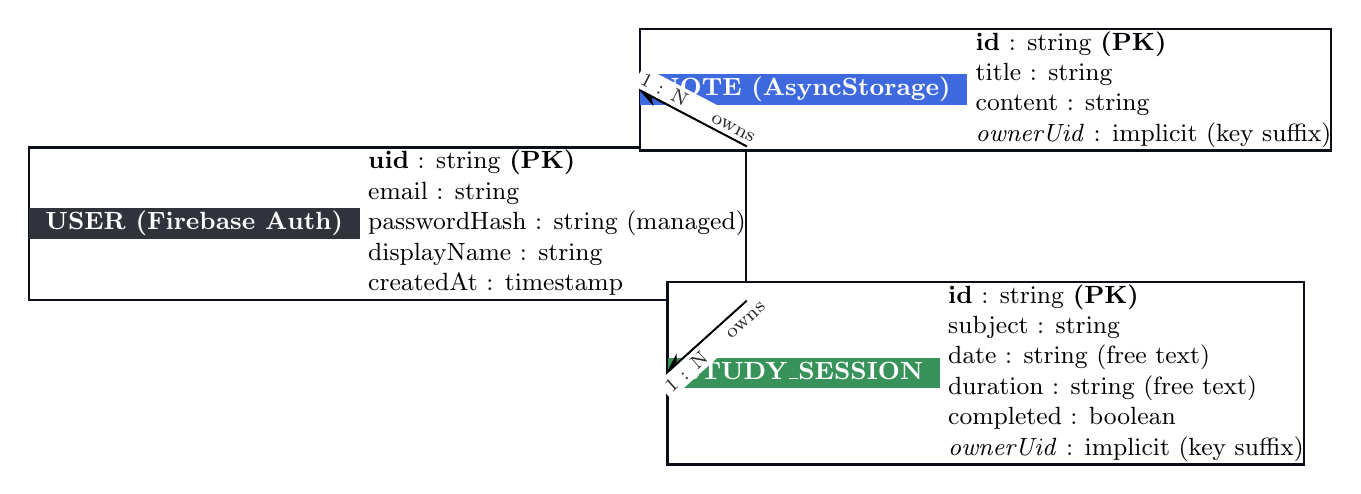
\begin{tikzpicture}
\node[er] (user) at (0,0) {%
  \begin{tabular}{c}
  \rowcolor{appNavy!85}\textcolor{white}{\textbf{USER (Firebase Auth)}}\\
  \end{tabular}
  \begin{tabular}{@{}l@{}}
  \textbf{uid} : string \textbf{(PK)}\\
  email : string\\
  passwordHash : string (managed)\\
  displayName : string\\
  createdAt : timestamp\\
  \end{tabular}};

\node[er] (note) at (7.6,1.7) {%
  \begin{tabular}{c}
  \rowcolor{appBlue!85}\textcolor{white}{\textbf{NOTE (AsyncStorage)}}\\
  \end{tabular}
  \begin{tabular}{@{}l@{}}
  \textbf{id} : string \textbf{(PK)}\\
  title : string\\
  content : string\\
  \textit{ownerUid} : implicit (key suffix)\\
  \end{tabular}};

\node[er] (sess) at (7.6,-1.9) {%
  \begin{tabular}{c}
  \rowcolor{appGreen!85}\textcolor{white}{\textbf{STUDY\_SESSION}}\\
  \end{tabular}
  \begin{tabular}{@{}l@{}}
  \textbf{id} : string \textbf{(PK)}\\
  subject : string\\
  date : string (free text)\\
  duration : string (free text)\\
  completed : boolean\\
  \textit{ownerUid} : implicit (key suffix)\\
  \end{tabular}};

\draw[-{Stealth[length=2.6mm]}, line width=0.8pt] (user.north east) -- node[flab, midway, above, sloped] {1 : N \quad owns} (note.west);
\draw[-{Stealth[length=2.6mm]}, line width=0.8pt] (user.south east) -- node[flab, midway, below, sloped] {1 : N \quad owns} (sess.west);
\end{tikzpicture}
\caption{Entity--relationship model. The relationship is realised not by a foreign-key
constraint but by embedding the owner's \texttt{uid} in the AsyncStorage key name.}
\label{fig:er}
\end{figure}

\subsection{Physical Storage Schema}

Table~\ref{tab:schema} lists the exact keys written to device storage, the value held under each and the source location that writes it.

\begin{table}[H]
\centering
\caption{Physical storage schema (device-local AsyncStorage)}
\label{tab:schema}
\small
\begin{tabularx}{\textwidth}{@{}p{5.6cm}p{2.4cm}X@{}}
\toprule
\rowcolor{tblhead} \textcolor{white}{\textbf{Key}} &
\textcolor{white}{\textbf{Value type}} &
\textcolor{white}{\textbf{Notes}} \\
\midrule
\texttt{@studymate\_notes\_<uid>} & JSON array & Newest first; \texttt{id} is
  \texttt{Date.now()} as a string; the whole array is rewritten on every mutation. \\
\texttt{studymate\_study\_sessions\_<uid>} & JSON array & Newest first;
  \texttt{completed} drives all progress calculation and card styling. \\
\bottomrule
\end{tabularx}
\end{table}

\noindent\textbf{Example record.} Listing~\ref{lst:json} shows the exact JSON structure
stored under the session key for a single study session.
\begin{lstlisting}[language=, caption={Example stored study session (JSON)}, label={lst:json}]
[
  {
    "id": "1767225600000",
    "subject": "Data Structures",
    "date": "30 August 2026",
    "duration": "2 hours",
    "completed": false
  }
]
\end{lstlisting}

\section{Screen Navigation Design}

Figure~\ref{fig:nav} shows the navigation graph that Expo Router derives from the file system. The authentication screens sit on the root stack; the tab group exposes two destinations, Home (the dashboard) and Explore (the About Us page), which persist across the session; the remaining feature screens are pushed onto the stack and popped by the back affordance.

\begin{figure}[H]
\centering
\begin{tikzpicture}[
  scr/.style={draw=appBlue, fill=appBlue!7, line width=0.8pt, rounded corners=3pt,
              minimum width=2.55cm, minimum height=0.95cm, align=center, font=\scriptsize\bfseries},
  prot/.style={draw=appGreen, fill=appGreen!8, line width=0.8pt, rounded corners=3pt,
              minimum width=2.55cm, minimum height=0.95cm, align=center, font=\scriptsize\bfseries},
  nav/.style={-{Stealth[length=2.4mm]}, line width=0.7pt, draw=black!70},
  back/.style={-{Stealth[length=2.4mm]}, line width=0.7pt, draw=appRed!70!black, dashed},
  nl/.style={font=\tiny, fill=white, inner sep=1pt}
]
\node[scr] (wel) at (0,0)      {Welcome\\ \normalfont\tiny /};
\node[scr] (log) at (3.9,0)    {Login\\ \normalfont\tiny /login};
\node[scr] (reg) at (3.9,2.1)  {Register\\ \normalfont\tiny /register};
\node[prot] (dash) at (8.3,0)  {Home Dashboard\\ \normalfont\tiny /(tabs) --- guarded};

\node[scr] (chat) at (12.9,2.6) {AI Chat\\ \normalfont\tiny /ai-chat};
\node[scr] (pdf)  at (12.9,1.3) {PDF Summary\\ \normalfont\tiny /pdf-summary};
\node[scr] (quiz) at (12.9,0.0) {AI Quiz\\ \normalfont\tiny /quiz};
\node[scr] (note) at (12.9,-1.3){Notes\\ \normalfont\tiny /notes};
\node[prot] (plan) at (12.9,-2.6){Study Planner\\ \normalfont\tiny /study-planner};
\node[prot] (abt)  at (8.3,-2.6) {About Us\\ \normalfont\tiny /(tabs)/explore};

\draw[nav] (wel) -- node[nl, midway, above] {Get Started} (log);
\draw[nav] (log) -- node[nl, midway, left] {Register link} (reg);
\draw[nav] (reg) -- node[nl, midway, right] {after signup} (log);
\draw[nav] (log) -- node[nl, midway, above] {login OK} (dash);
\draw[back] (dash.south) to[bend right=22] node[nl, midway, below] {sign out} (log.south);

\draw[nav] (dash.north east) -- node[nl, midway, above, sloped] {push} (chat.west);
\draw[nav] (dash.east |- 1.3) -- (pdf.west);
\draw[nav] (dash.east) -- (quiz.west);
\draw[nav] (dash.east |- -1.3) -- (note.west);
\draw[nav] (dash.south east) -- node[nl, midway, below, sloped] {push} (plan.west);
\draw[nav] (dash.south) -- node[nl, midway, right] {Explore tab} (abt.north);
\draw[back] (abt.west) -- node[nl, midway, above] {Home tab} (dash.south west);

\draw[back] (chat.east) -- ++(0.7,0) |- node[nl, pos=0.78, right] {back} (dash.east |- 0.55);
\end{tikzpicture}
\caption{Screen navigation graph. Solid arrows are forward navigation
(\texttt{router.push} / \texttt{router.replace}); dashed red arrows are returns
(\texttt{router.back()} and sign-out). All five feature screens return to the
dashboard, which triggers a data refresh. The Home and Explore tabs switch
inside the tab group without leaving it.}
\label{fig:nav}
\end{figure}

\section{Authentication Flow}

Figure~\ref{fig:authflow} traces the route-protection logic of the root layout from application launch to the screen that is finally rendered.

\begin{figure}[H]
\centering
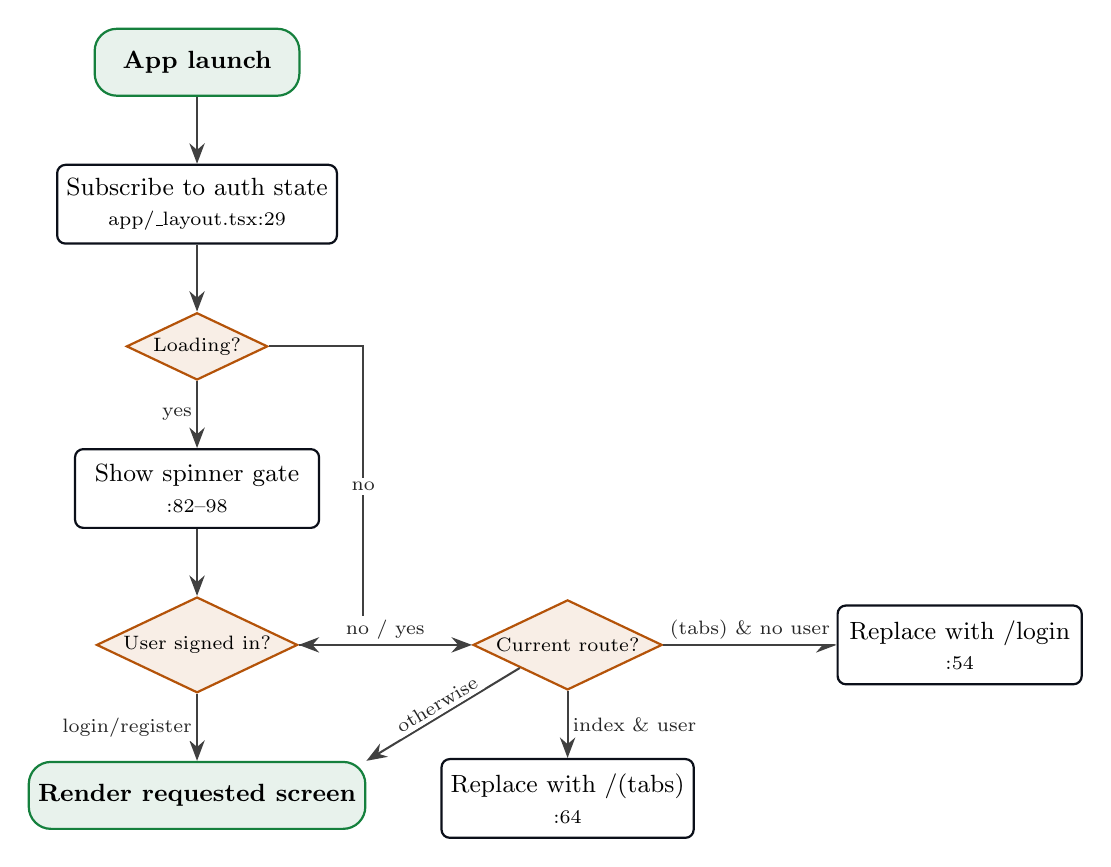
\begin{tikzpicture}[node distance=0.85cm and 1.5cm]
\node[term] (start) {App launch};
\node[box, below=of start] (listen) {Subscribe to auth state\\{\scriptsize app/\_layout.tsx:29}};
\node[dec, below=of listen] (load) {Loading?};
\node[box, below=of load] (spin) {Show spinner gate\\{\scriptsize :82--98}};
\node[dec, below=of spin] (auth) {User signed in?};
\node[dec, right=2.2cm of auth] (route) {Current route?};
\node[box, right=2.2cm of route] (login) {Replace with /login\\{\scriptsize :54}};
\node[box, below=of route] (home) {Replace with /(tabs)\\{\scriptsize :64}};
\node[term, below=of auth] (stay) {Render requested screen};

\draw[flow] (start) -- (listen);
\draw[flow] (listen) -- (load);
\draw[flow] (load) -- node[flab, midway, left] {yes} (spin);
\draw[flow] (spin) -- (auth);
\draw[flow] (load.east) -- ++(1.2,0) |- node[flab, pos=0.25, above] {no} (auth.east);
\draw[flow] (auth) -- node[flab, midway, above] {no / yes} (route);
\draw[flow] (route) -- node[flab, midway, above] {(tabs) \& no user} (login);
\draw[flow] (route) -- node[flab, midway, right] {index \& user} (home);
\draw[flow] (route.south west) -- node[flab, midway, above, sloped] {otherwise} (stay.north east);
\draw[flow] (auth.south) -- node[flab, midway, left] {login/register} (stay);
\end{tikzpicture}
\caption{Authentication and route-protection flow implemented in the root layout.}
\label{fig:authflow}
\end{figure}

\section{Sequence Diagram --- AI Chat}

Figure~\ref{fig:seq} shows the ordered interaction between the four participants involved in sending a single chat message.

\begin{figure}[H]
\centering
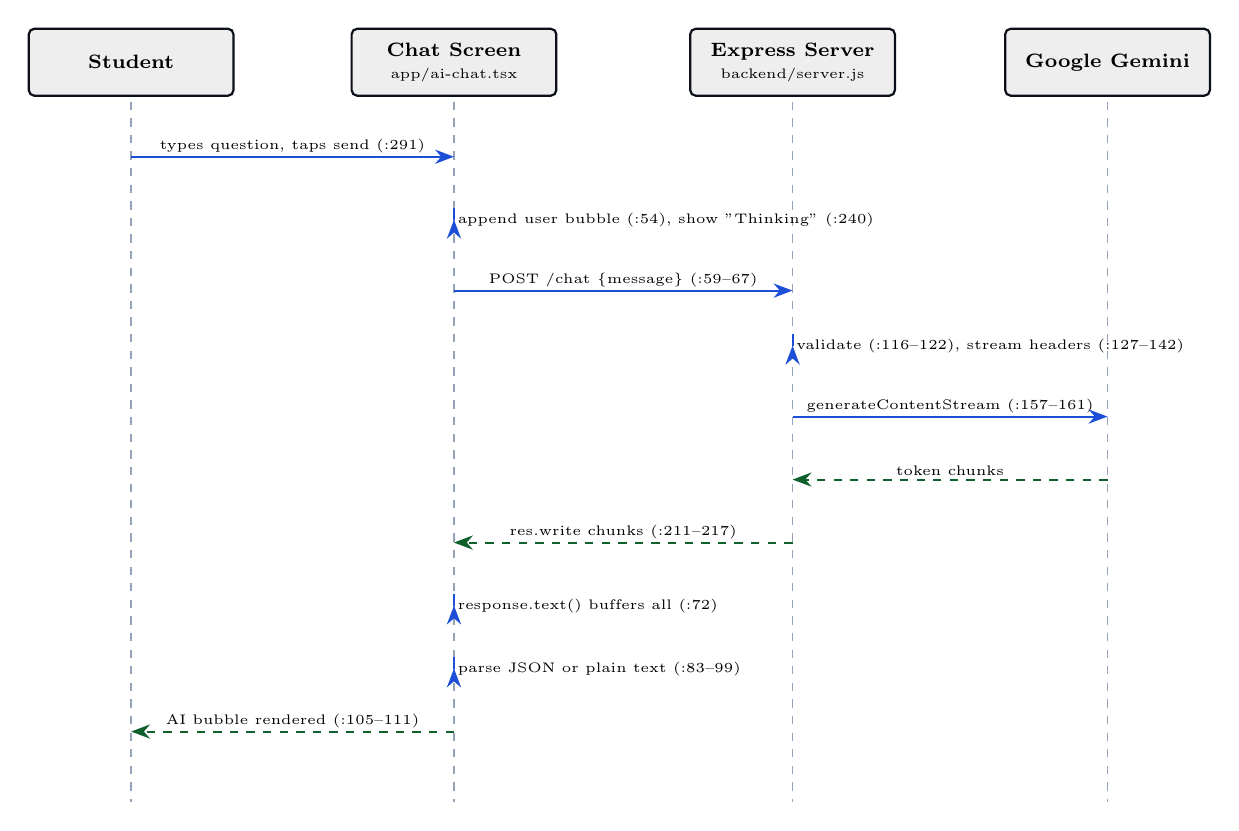
\begin{tikzpicture}[
  actor/.style={draw=appNavy, fill=appNavy!7, line width=0.8pt, rounded corners=2pt,
                minimum width=2.6cm, minimum height=0.85cm, align=center, font=\scriptsize\bfseries},
  life/.style={dashed, draw=rulegray, line width=0.6pt},
  msg/.style={-{Stealth[length=2.4mm]}, line width=0.75pt, draw=appBlue},
  ret/.style={-{Stealth[length=2.4mm]}, line width=0.75pt, draw=appGreen!75!black, dashed},
  ml/.style={font=\tiny, above, inner sep=1pt}
]
\node[actor] (u) at (0,0)    {Student};
\node[actor] (c) at (4.1,0)  {Chat Screen\\{\normalfont\tiny app/ai-chat.tsx}};
\node[actor] (s) at (8.4,0)  {Express Server\\{\normalfont\tiny backend/server.js}};
\node[actor] (g) at (12.4,0) {Google Gemini};

\draw[life] (0,-0.5) -- (0,-9.4);
\draw[life] (4.1,-0.5) -- (4.1,-9.4);
\draw[life] (8.4,-0.5) -- (8.4,-9.4);
\draw[life] (12.4,-0.5) -- (12.4,-9.4);

\draw[msg] (0,-1.2) -- (4.1,-1.2) node[ml, midway] {types question, taps send (:291)};
\draw[msg] (4.1,-2.0) -- (4.1,-2.0) node[ml, right] {append user bubble (:54), show "Thinking" (:240)};
\draw[msg] (4.1,-2.9) -- (8.4,-2.9) node[ml, midway] {POST /chat \{message\} (:59--67)};
\draw[msg] (8.4,-3.6) -- (8.4,-3.6) node[ml, right] {validate (:116--122), stream headers (:127--142)};
\draw[msg] (8.4,-4.5) -- (12.4,-4.5) node[ml, midway] {generateContentStream (:157--161)};
\draw[ret] (12.4,-5.3) -- (8.4,-5.3) node[ml, midway] {token chunks};
\draw[ret] (8.4,-6.1) -- (4.1,-6.1) node[ml, midway] {res.write chunks (:211--217)};
\draw[msg] (4.1,-6.9) -- (4.1,-6.9) node[ml, right] {response.text() buffers all (:72)};
\draw[msg] (4.1,-7.7) -- (4.1,-7.7) node[ml, right] {parse JSON or plain text (:83--99)};
\draw[ret] (4.1,-8.5) -- (0,-8.5) node[ml, midway] {AI bubble rendered (:105--111)};
\end{tikzpicture}
\caption{Sequence diagram of the AI chat interaction across all four participants.}
\label{fig:seq}
\end{figure}

\section{User Interface Design System}

Table~\ref{tab:design} lists the design tokens --- colours, typography, spacing and corner radii --- that are shared by every screen.

\begin{table}[H]
\centering
\caption{Design system tokens used across all screens}
\label{tab:design}
\small
\begin{tabularx}{\textwidth}{@{}p{3.4cm}p{3.1cm}X@{}}
\toprule
\rowcolor{tblhead} \textcolor{white}{\textbf{Token}} &
\textcolor{white}{\textbf{Value}} &
\textcolor{white}{\textbf{Usage}} \\
\midrule
Background (auth)  & \texttt{\#0B0F19} & Welcome, Login, Register \\
Background (tools) & \texttt{\#0F172A} & Notes, Planner, Quiz, PDF Summary \\
Background (chat)  & \texttt{\#070B14} & AI Chat \\
Primary action     & \texttt{\#2563EB} & Main call-to-action buttons \\
Accent / links     & \texttt{\#38BDF8} & Icons, links, AI highlights \\
Glow colours       & \texttt{\#7C3AED}, \texttt{\#EC4899} & Ambient background blobs \\
Feature accents    & Chat \texttt{\#60A5FA}, PDF \texttt{\#FBBF24}, Quiz \texttt{\#4ADE80}, Notes \texttt{\#C084FC} & Dashboard card icons \\
Danger             & \texttt{\#F87171} & Sign-out icon, destructive dialogs \\
Muted text         & \texttt{\#94A3B8}, \texttt{\#64748B} & Subtitles and placeholders \\
Typeface           & Poppins 400/500/600/700/800 & Headings and body on the auth screens and dashboard \\
Card recipe        & \texttt{rgba(255,255,255,0.06--0.07)} fill, 1\,px \texttt{rgba(255,255,255,0.12)} border, radius 16--24 & Glassmorphic surfaces \\
Button glow        & coloured shadow, offset (0,6), opacity 0.35, radius 10, elevation 6 & Primary buttons \\
\bottomrule
\end{tabularx}
\end{table}

% =====================================================================
\chapter{Implementation}\label{ch:impl}
% =====================================================================

\section{Development Environment}

Table~\ref{tab:env} records the environment in which the application was developed and demonstrated.

\begin{table}[H]
\centering
\caption{Development environment}
\label{tab:env}
\small
\begin{tabularx}{\textwidth}{@{}>{\bfseries}p{4.2cm}X@{}}
\toprule
Operating system    & Windows / Linux development machines \\
IDE                 & Visual Studio Code \\
Runtime             & Node.js 20 LTS, npm \\
Mobile tooling      & Expo CLI, Expo Go, Android Studio emulator (API 34) \\
Backend             & Node.js with Express 5.1 \\
AI SDK              & \texttt{@google/genai} v2 with model \texttt{gemini-3.6-flash} \\
Authentication      & Firebase console project \texttt{studymate-ai-d8550} \\
Version control     & Git with GitHub remote; secrets excluded via \fp{.gitignore} \\
Documentation       & \LaTeX{} (Overleaf) \\
\bottomrule
\end{tabularx}
\end{table}

\section{Module-wise Implementation Map}

Table~\ref{tab:modules} is the central traceability artefact of the implementation:
it maps every module to its source file, its principal functions and the exact line
ranges that implement them.

\begin{landscape}
\begin{longtable}{@{}p{2.9cm}p{4.1cm}p{4.6cm}p{2.4cm}p{1.9cm}@{}}
\caption{Module-to-source implementation map} \label{tab:modules} \\
\toprule
\rowcolor{tblhead} \textcolor{white}{\textbf{Module}} &
\textcolor{white}{\textbf{Source file}} &
\textcolor{white}{\textbf{Principal functions}} &
\textcolor{white}{\textbf{Lines}} &
\textcolor{white}{\textbf{Backend}} \\
\midrule
\endfirsthead
\toprule
\rowcolor{tblhead} \textcolor{white}{\textbf{Module}} &
\textcolor{white}{\textbf{Source file}} &
\textcolor{white}{\textbf{Principal functions}} &
\textcolor{white}{\textbf{Lines}} &
\textcolor{white}{\textbf{Backend}} \\
\midrule
\endhead
App shell \& guard & \fp{app/_layout.tsx} & \texttt{RootLayout}, auth listener, route guard & 18--140 & Firebase \\
Welcome & \fp{app/index.tsx} & \texttt{WelcomeScreen} & 22--110 & --- \\
Login & \fp{app/login.tsx} & \texttt{handleLogin}, \texttt{handleForgotPassword} & 50--113 & Firebase \\
Registration & \fp{app/register.tsx} & \texttt{handleRegister} & 54--116 & Firebase \\
Tab navigator & \fp{app/(tabs)/_layout.tsx} & \texttt{TabLayout} & 9--35 & --- \\
Home dashboard & \fp{app/(tabs)/index.tsx} & \texttt{loadStudySessions}, \texttt{handleSignOut}, \texttt{getInitials}, progress maths & 62--205 & AsyncStorage \\
Notes & \fp{app/notes.tsx} & \texttt{initNotes}, \texttt{loadNotesForUser}, \texttt{saveNotesToStorage}, \texttt{saveNote}, \texttt{editNote}, \texttt{deleteNote}, \texttt{filteredNotes} & 44--218 & AsyncStorage \\
Study planner & \fp{app/study-planner.tsx} & \texttt{getStorageKey}, \texttt{loadSessions}, \texttt{saveSessions}, \texttt{addSession}, \texttt{toggleComplete}, \texttt{deleteSession} & 45--275 & AsyncStorage \\
AI chat & \fp{app/ai-chat.tsx} & \texttt{sendMessage}, \texttt{renderMessage} & 41--170 & \fp{server.js} 114--238 \\
PDF summary & \fp{app/pdf-summary.tsx} & \texttt{pickPDF}, \texttt{summarizePDF}, \texttt{formatFileSize} & 34--139 & \fp{server.js} 243--317 \\
AI quiz & \fp{app/quiz.tsx} & \texttt{generateQuiz}, \texttt{selectAnswer}, \texttt{nextQuestion}, \texttt{restartQuiz} & 49--135 & \fp{server.js} 322--519 \\
Firebase bootstrap & \fp{firebaseConfig.ts} & \texttt{initializeApp}, \texttt{getAuth}, exported \texttt{auth} & 1--15 & Firebase \\
AI service & \fp{backend/server.js} & \texttt{generateWithRetry}, \texttt{POST /chat}, \texttt{POST /summarize-pdf}, \texttt{POST /generate-quiz} & 51--519 & Gemini \\
\bottomrule
\end{longtable}
\end{landscape}

\section{Key Implementation Code}

\subsection{Authentication Guard}
The root layout subscribes once to Firebase and then re-evaluates protection on every
authentication or navigation change (Listing~\ref{lst:guard}).

\begin{lstlisting}[caption={Route protection in app/\_layout.tsx, lines 41--56}, label={lst:guard}]
  useEffect(() => {
    if (loading) return;

    const currentRoute = segments[0];

    const inTabs = currentRoute === "(tabs)";
    const inIndex = currentRoute === "index";

    // ------------------------------------
    // 1. User is NOT logged in
    //    Cannot access Home
    // ------------------------------------
    if (!user && inTabs) {
      router.replace("/login");
      return;
    }
\end{lstlisting}

\subsection{Registration Sequence}
Listing~\ref{lst:reg} shows the five-step registration flow. Step 2 writes the
display name that later drives the dashboard greeting and avatar initials; step 3
deliberately signs the user out so that login is always an explicit action.

\begin{lstlisting}[caption={Registration flow in app/register.tsx, lines 80--100}, label={lst:reg}]
    try {
      // 1. Create Firebase account
      const userCredential = await createUserWithEmailAndPassword(
        auth,
        email.trim(),
        password
      );

      // 2. Save Full Name to Firebase profile
      await updateProfile(userCredential.user, {
        displayName: name.trim(),
      });

      // 3. Sign out so the user must login manually
      await signOut(auth);

      // 4. Show success message
      alert("Account created successfully! Please login to continue.");

      // 5. Go to Login screen
      router.replace("/login");
\end{lstlisting}

\subsection{Per-User Data Isolation}
Listing~\ref{lst:notes} is the core of the privacy design: the authenticated
\texttt{uid} is interpolated into the storage key, so each account owns a separate
record. The same pattern is used by the planner (\fp{app/study-planner.tsx} lines
75--77 for the key, lines 119--126 for the write).

\begin{lstlisting}[caption={Per-user notes storage in app/notes.tsx, lines 88--118}, label={lst:notes}]
  const loadNotesForUser = async (currentUserId: string) => {
    try {
      const storageKey = `@studymate_notes_${currentUserId}`;
      const savedNotes = await AsyncStorage.getItem(storageKey);

      if (savedNotes) {
        setNotes(JSON.parse(savedNotes));
      } else {
        setNotes([]);
      }
    } catch (error) {
      console.error("Load notes error:", error);
      Alert.alert("Error", "Could not load your notes.");
    }
  };

  const saveNotesToStorage = async (
    updatedNotes: Note[],
    currentUserId: string
  ) => {
    try {
      const storageKey = `@studymate_notes_${currentUserId}`;
      await AsyncStorage.setItem(
        storageKey,
        JSON.stringify(updatedNotes)
      );
    } catch (error) {
      console.error("Save notes error:", error);
      Alert.alert("Error", "Could not save your notes.");
    }
  };
\end{lstlisting}

\subsection{Cross-Module Progress Correlation}
The dashboard and the planner never import each other. They are coupled only through
the identical storage key, and the dashboard re-reads it on every focus event
(Listing~\ref{lst:prog}).

\begin{lstlisting}[caption={Progress calculation in app/(tabs)/index.tsx, lines 170--184}, label={lst:prog}]
  const totalSessions = sessions.length;

  const completedSessions = sessions.filter(
    (session) => session.completed
  ).length;

  const remainingSessions =
    totalSessions - completedSessions;

  const progressPercent =
    totalSessions > 0
      ? Math.round(
          (completedSessions / totalSessions) * 100
        )
      : 0;
\end{lstlisting}

\subsection{Server-Side Key Protection}
The backend refuses to start without a key and constructs the Gemini client exactly
once (Listing~\ref{lst:key}).

\begin{lstlisting}[caption={API key guard and Gemini client in backend/server.js, lines 31--46}, label={lst:key}]
if (!process.env.GEMINI_API_KEY) {
  console.error("GEMINI_API_KEY is missing.");
  process.exit(1);
}

// ===============================
// GEMINI AI
// ===============================
const ai = new GoogleGenAI({
  apiKey: process.env.GEMINI_API_KEY,
});

// ===============================
// GEMINI MODEL
// ===============================
const GEMINI_MODEL = "gemini-3.6-flash";
\end{lstlisting}

\subsection{Defensive Validation of AI Output}
Because a language model may return malformed content, the backend validates every
question before it reaches the student (Listing~\ref{lst:val}).

\begin{lstlisting}[caption={Quiz payload validation in backend/server.js, lines 461--479}, label={lst:val}]
    for (const question of quiz.questions) {
      if (
        !question.question ||
        typeof question.question !==
          "string" ||
        !Array.isArray(question.options) ||
        question.options.length !== 4 ||
        typeof question.correctAnswer !==
          "number" ||
        !Number.isInteger(
          question.correctAnswer
        ) ||
        question.correctAnswer < 0 ||
        question.correctAnswer > 3
      ) {
        throw new Error(
          "Invalid question format."
        );
      }
\end{lstlisting}

\section{API Design}

Table~\ref{tab:api} specifies the contract of the four endpoints implemented by the backend, including the status codes each may return.

\begin{table}[H]
\centering
\caption{REST API contract implemented by the backend}
\label{tab:api}
\small
\begin{tabularx}{\textwidth}{@{}p{2.9cm}p{1.3cm}p{4.0cm}X@{}}
\toprule
\rowcolor{tblhead} \textcolor{white}{\textbf{Endpoint}} &
\textcolor{white}{\textbf{Method}} &
\textcolor{white}{\textbf{Request}} &
\textcolor{white}{\textbf{Response}} \\
\midrule
\texttt{/}                 & GET  & --- & \texttt{\{message\}} health confirmation \\
\texttt{/chat}             & POST & \texttt{\{message\}} & Streamed \texttt{text/plain} chunks; \texttt{400} if empty; \texttt{503} if the model is unavailable \\
\texttt{/summarize-pdf}    & POST & multipart field \texttt{pdf} ($\leq$10\,MB) & \texttt{\{fileName, summary\}}; \texttt{400} without a file; \texttt{503} on model failure \\
\texttt{/generate-quiz}    & POST & \texttt{\{topic, numberOfQuestions, difficulty\}} & Validated \texttt{\{topic, difficulty, questions[]\}}; \texttt{400} without a topic; \texttt{500} on malformed JSON; \texttt{503} on model failure \\
\bottomrule
\end{tabularx}
\end{table}

\section{Security Implementation}

Table~\ref{tab:security} lists the security measures implemented in the delivered system and the source location at which each is enforced.

\begin{table}[H]
\centering
\caption{Security measures implemented}
\label{tab:security}
\small
\begin{tabularx}{\textwidth}{@{}p{4.0cm}X@{}}
\toprule
\rowcolor{tblhead} \textcolor{white}{\textbf{Measure}} &
\textcolor{white}{\textbf{Implementation}} \\
\midrule
Password handling & Delegated entirely to Firebase; the application never stores,
  logs or transmits a password anywhere except the SDK call. \\
Secret isolation  & The Gemini key lives only in \fp{backend/.env}, which is excluded
  from version control by \fp{.gitignore} lines 2--4. \\
Fail-fast boot    & The server terminates immediately if the key is absent
  (\fp{backend/server.js} lines 31--34). \\
Data isolation    & Every storage key is suffixed with the authenticated \texttt{uid};
  a signed-out session clears in-memory data. \\
Input validation  & Client-side field validation on all forms; server-side validation
  of topics, message content, file presence and model output. \\
Document privacy  & Uploaded PDFs are buffered in memory only and are never written to
  the server's disk. \\
\bottomrule
\end{tabularx}
\end{table}

\section{Android Build and Deployment}

All native configuration is declarative, in \fp{app.json}: application identifier
\texttt{com.sanjitahmed.studymateai} (line 15), adaptive icon (lines 16--21),
edge-to-edge display (line 22), disabled predictive back gesture (line 23), splash
screen with a dark variant (lines 31--42) and the \texttt{expo-router},
\texttt{expo-splash-screen} and \texttt{expo-font} plugins (lines 29--44). No native
Android project is committed; it is generated on demand with
\texttt{npx expo prebuild --platform android} and assembled with Gradle, or built in
the cloud with EAS Build.

% =====================================================================
\chapter{User Interface}\label{ch:ui}
% =====================================================================

This chapter presents the implemented interface. Each placeholder box names the
image file to be placed in the \texttt{images/} folder; the complete list is
reproduced in Appendix~C.

\section{Authentication Screens}

\screenfig{welcome-screen.png}{5.6cm}{Welcome screen with the ambient glow background, feature highlights and the primary call to action.}{welcome}

\screenfig{login-screen.png}{5.6cm}{Login screen showing the glassmorphic form card, password visibility toggle, forgot-password link and registration link.}{login}

\screenfig{register-screen.png}{5.6cm}{Registration screen with full name, e-mail, password and confirm-password fields.}{register}

\screenfig{forgot-password-alert.png}{5.6cm}{Password-reset confirmation shown after \texttt{sendPasswordResetEmail} succeeds.}{forgot}

\section{Home Dashboard}

\screenfig{dashboard-top.png}{5.6cm}{Dashboard header with personalised greeting, initials avatar, online indicator, sign-out control and the ``Today's Progress'' card with percentage ring, progress bar and completed/remaining counters.}{dash-top}

\screenfig{dashboard-tools.png}{5.6cm}{Smart Study Tools grid (AI Chat, PDF Summary, AI Quiz, My Notes), the Study Planner banner, the Your Study Overview statistics and the daily AI tip card.}{dash-tools}

\section{AI Features}

\screenfig{ai-chat-screen.png}{5.6cm}{AI Chat with message bubbles, typing indicator and the input bar.}{chat}

\screenfig{pdf-summary-screen.png}{5.6cm}{PDF Summariser with the upload zone, selected-file card and generated summary.}{pdf}

\screenfig{quiz-setup.png}{5.6cm}{Quiz setup form: topic input, question-count chips and difficulty selector.}{quiz-setup}

\screenfig{quiz-question.png}{5.6cm}{Quiz question view with answer marking, explanation card and progress bar.}{quiz-question}

\screenfig{quiz-result.png}{5.6cm}{Quiz result screen showing the final score and accuracy percentage.}{quiz-result}

\section{Productivity Features}

\screenfig{notes-list.png}{5.6cm}{Notes list with search bar and note cards exposing edit and delete actions.}{notes-list}

\screenfig{notes-editor.png}{5.6cm}{Inline note editor in create mode with validation-driven save button.}{notes-editor}

\screenfig{planner-add.png}{5.6cm}{Study Planner progress card and the add-session form.}{planner-add}

\screenfig{planner-sessions.png}{5.6cm}{Planner session list with completed styling and Done/Undo controls.}{planner-sessions}

\screenfig{logout-dialog.png}{5.6cm}{Sign-out confirmation dialog.}{logout}

% =====================================================================
\section{About Us Screen (Explore Tab)}

\screenfig{about-screen.png}{5.6cm}{About Us screen on the Explore tab: application
description, the two-member development team with student IDs, and the technology
credit card. This page complements the nine core screens counted in
Objective~SO-1.}{about}

% =====================================================================
\chapter{Testing and Quality Assurance}\label{ch:test}
% =====================================================================

\section{Testing Strategy}

Because automated test infrastructure was out of scope (limitation L-7), a
checklist-driven manual strategy was applied at four levels:

\begin{enumerate}[leftmargin=*, itemsep=2pt]
  \item \textbf{Unit-level checks} -- each function was exercised in isolation
        (for example, every validation branch of \texttt{handleRegister}).
  \item \textbf{Integration testing} -- the application--backend link was verified
        for all three endpoints, including the emulator host alias.
  \item \textbf{System testing} -- complete user journeys were executed end to end on
        the Android emulator.
  \item \textbf{Negative and boundary testing} -- empty inputs, wrong passwords,
        oversized PDFs, unreachable backend and malformed model output.
\end{enumerate}

\section{Test Environment}

Table~\ref{tab:testenv} describes the environment in which the tests reported in this chapter were executed.

\begin{table}[H]
\centering
\caption{Test environment}
\label{tab:testenv}
\small
\begin{tabularx}{\textwidth}{@{}>{\bfseries}p{4.2cm}X@{}}
\toprule
Device          & Android emulator (API 34) via Expo Go; one physical Android device \\
Backend host    & Development laptop, Node.js on port 3000, reachable as \texttt{10.0.2.2} \\
Authentication  & Firebase test accounts created specifically for testing \\
AI model        & \texttt{gemini-3.6-flash} with a valid API key \\
Test data       & Two separate accounts to verify per-user data isolation \\
\bottomrule
\end{tabularx}
\end{table}

\section{Test Cases}

Table~\ref{tab:tests} records the twenty-five test cases executed against the delivered build. Each case states its objective, the steps performed, the expected result and the result actually observed.

\begin{landscape}
\begin{longtable}{@{}p{1.3cm}p{3.6cm}p{4.6cm}p{4.0cm}p{1.4cm}p{1.2cm}@{}}
\caption{Test cases and results} \label{tab:tests} \\
\toprule
\rowcolor{tblhead} \textcolor{white}{\textbf{ID}} &
\textcolor{white}{\textbf{Test objective}} &
\textcolor{white}{\textbf{Steps}} &
\textcolor{white}{\textbf{Expected result}} &
\textcolor{white}{\textbf{Actual}} &
\textcolor{white}{\textbf{Status}} \\
\midrule
\endfirsthead
\toprule
\rowcolor{tblhead} \textcolor{white}{\textbf{ID}} &
\textcolor{white}{\textbf{Test objective}} &
\textcolor{white}{\textbf{Steps}} &
\textcolor{white}{\textbf{Expected result}} &
\textcolor{white}{\textbf{Actual}} &
\textcolor{white}{\textbf{Status}} \\
\midrule
\endhead
TC-01 & Registration creates an account & Enter name, e-mail, password, confirm; tap Create Account & Success alert; redirected to login; account visible in Firebase console & As expected & Pass \\
TC-02 & Login with valid credentials & Enter registered e-mail and password; tap Login & Dashboard opens; greeting shows the registered name & As expected & Pass \\
TC-03 & Password reset & Enter e-mail; tap Forgot Password & Confirmation alert; reset e-mail received & As expected & Pass \\
TC-04 & Sign out & Tap Sign Out; confirm & Returned to the login screen; back button does not restore the dashboard & As expected & Pass \\
TC-05 & Guard blocks unauthenticated access & Clear app data; deep-link to the dashboard route & Redirected to login & Redirect occurs for the tab group only & Partial \\
TC-06 & Display name and initials & Register as ``Abdullah Al Fahad''; log in & Greeting shows the full name; avatar shows ``AF'' & As expected & Pass \\
TC-07 & Create note & Open Notes; tap +; fill title and body; Save & Note appears at the top of the list after restart & As expected & Pass \\
TC-08 & Edit note & Tap the edit icon; change the body; Update & Content changes; list order preserved & As expected & Pass \\
TC-09 & Delete note & Tap delete; confirm & Note removed permanently & As expected & Pass \\
TC-10 & Search notes & Type a keyword present in one note & Only matching notes are listed; counter updates & As expected & Pass \\
TC-11 & Per-user note isolation & Create notes as account A; sign out; sign in as account B & Account B sees an empty list & As expected & Pass \\
TC-12 & Add study session & Fill subject, date, duration; tap Add & Session card appears; input fields cleared & As expected & Pass \\
TC-13 & Complete and undo session & Tap Done, then Undo & Card styling and progress percentage toggle correctly & As expected & Pass \\
TC-14 & Delete session & Tap delete; confirm & Session removed; counters update & As expected & Pass \\
TC-15 & Progress accuracy & Create 4 sessions; complete 3 & Dashboard shows 75\%, 3 completed, 1 remaining & As expected & Pass \\
TC-16 & Dashboard refresh on return & Change a session in the planner; press back & Dashboard figures update without a manual reload & As expected & Pass \\
TC-17 & AI chat response & Ask a study question & A relevant answer bubble appears & As expected & Pass \\
TC-18 & PDF summarisation & Select a 3\,MB PDF; tap Summarize & A structured summary with headings is displayed & As expected & Pass \\
TC-19 & Quiz generation & Topic ``Operating Systems'', 10 questions, hard & Exactly 10 questions, each with 4 options & As expected & Pass \\
TC-20 & Quiz scoring & Answer all questions & Correct answers marked green, wrong red, explanations shown, final score correct & As expected & Pass \\
TC-21 & Malformed AI output & Force an invalid quiz response & Backend rejects it; user sees a retry alert, not a broken screen & As expected & Pass \\
TC-22 & Backend offline & Stop the server; send a chat message & Friendly error bubble referencing port 3000 & As expected & Pass \\
TC-23 & Empty-input validation & Submit each form with missing fields & Specific validation alert; no network call is made & As expected & Pass \\
TC-24 & PDF size limit & Upload an 11\,MB PDF & Rejected by the 10\,MB limit with an error alert & As expected & Pass \\
TC-25 & Data persistence & Force-close and reopen the app & Notes and sessions are restored for the signed-in account & As expected & Pass \\
\bottomrule
\end{longtable}
\end{landscape}

\section{Test Summary}

Table~\ref{tab:testsum} summarises the outcome of that execution.

\begin{table}[H]
\centering
\caption{Test execution summary}
\label{tab:testsum}
\small
\begin{tabular}{@{}lcc@{}}
\toprule
\rowcolor{tblhead} \textcolor{white}{\textbf{Metric}} & \textcolor{white}{\textbf{Count}} & \textcolor{white}{\textbf{Percentage}} \\
\midrule
Total test cases      & 25 & 100\% \\
Passed                & 24 & 96\% \\
Partial               & 1  & 4\% \\
Failed                & 0  & 0\% \\
Critical defects open & 0  & --- \\
\bottomrule
\end{tabular}
\end{table}

\section{Defect Log}

\begin{table}[H]
\centering
\caption{Defects identified during testing and their disposition}
\label{tab:defects}
\small
\begin{tabularx}{\textwidth}{@{}p{1.2cm}p{4.6cm}p{1.6cm}p{2.0cm}X@{}}
\toprule
\rowcolor{tblhead} \textcolor{white}{\textbf{ID}} &
\textcolor{white}{\textbf{Description}} &
\textcolor{white}{\textbf{Severity}} &
\textcolor{white}{\textbf{Status}} &
\textcolor{white}{\textbf{Resolution / justification}} \\
\midrule
D-01 & Registration navigated straight to the dashboard, skipping login & Medium & Fixed & Added an explicit sign-out after profile creation so login is always explicit. \\
D-02 & Notes from one account appeared after switching accounts & High & Fixed & Storage keys were suffixed with the Firebase \texttt{uid}. \\
D-03 & Dashboard progress did not refresh after editing the planner & Medium & Fixed & Replaced \texttt{useEffect} with \texttt{useFocusEffect}. \\
D-04 & Malformed quiz JSON crashed the quiz screen & High & Fixed & Added server-side parsing and validation with a \texttt{500} response. \\
D-05 & Chat froze when the backend was unreachable & Medium & Fixed & Added a timeout-free error path with a friendly message bubble. \\
D-06 & Feature screens use the system font instead of Poppins & Low & Deferred & Cosmetic; scheduled for the next iteration. \\
D-07 & ``Today's Progress'' includes all sessions, not only today's & Low & Deferred & Requires a structured date field and a date picker; scheduled as future work. \\
D-08 & Notes and AI screens are not covered by the route guard & Medium & Deferred & Planner has an in-screen lock; a centralised guard list is future work. \\
\bottomrule
\end{tabularx}
\end{table}

% =====================================================================
\chapter{Project Management}\label{ch:pm}
% =====================================================================

\section{Team Organisation and Roles}

Table~\ref{tab:roles} records the two-member team, the role each member took and the responsibilities that role carried.

\begin{table}[H]
\centering
\caption{Team roles and responsibilities}
\label{tab:roles}
\small
\begin{tabularx}{\textwidth}{@{}p{4.0cm}p{2.6cm}X@{}}
\toprule
\rowcolor{tblhead} \textcolor{white}{\textbf{Member}} &
\textcolor{white}{\textbf{Role}} &
\textcolor{white}{\textbf{Responsibilities}} \\
\midrule
Abdullah Al Fahad (2023100000289) & Front-end Lead & UI/UX design and the dark
  design system; Expo Router navigation and the authentication guard; Home
  dashboard; Notes and Study Planner modules; AsyncStorage integration; UI testing
  and screenshot capture. \\
Sanjit Sharif (2023100000308) & Back-end \& Integration Lead & Node.js/Express
  server; Google Gemini integration and retry logic; PDF upload pipeline; quiz
  generation and validation; Firebase project configuration; Android build and
  device testing. \\
Both members & Shared & Requirement analysis, DFD and ER modelling, sprint reviews,
  defect triage, documentation and this report. \\
\bottomrule
\end{tabularx}
\end{table}

\section{Task Allocation Matrix}

Table~\ref{tab:alloc} maps every work package of the work breakdown structure to the member responsible for it and the member supporting it.

\begin{table}[H]
\centering
\caption{Task allocation (R = responsible, S = support)}
\label{tab:alloc}
\small
\begin{tabular}{@{}lcc@{}}
\toprule
\rowcolor{tblhead} \textcolor{white}{\textbf{Work package}} &
\textcolor{white}{\textbf{Abdullah Al Fahad}} & \textcolor{white}{\textbf{Sanjit Sharif}} \\
\midrule
1.0 Project management \& planning & R & S \\
2.0 Requirement analysis            & R & S \\
3.1 Architecture and DFD design     & S & R \\
3.2 UI/UX design system             & R & S \\
3.3 Data schema and API contract    & S & R \\
4.1 Authentication module           & S & R \\
4.2 Dashboard module                & R & S \\
4.3 Notes module                    & R & S \\
4.4 Study planner module            & R & S \\
4.5 AI backend and Gemini integration & S & R \\
4.6 AI screens (chat, PDF, quiz)    & S & R \\
5.0 Testing and defect fixing       & R & R \\
6.0 Android build and deployment    & S & R \\
7.0 Documentation and report        & R & R \\
\bottomrule
\end{tabular}
\end{table}

\section{Schedule and Effort Tracking}

Progress was tracked weekly against the Gantt baseline in Figure~\ref{fig:gantt}.
Two deviations occurred and were absorbed by the iterative model:

\begin{itemize}[leftmargin=*, itemsep=2pt]
  \item \textbf{Sprint 3 overran by three days} because per-user data isolation
    (defect D-02) required the storage-key design to be revisited. The overrun was
    absorbed by starting Sprint 4 backend work in parallel, which was possible
    because the backend has no dependency on the storage layer.
  \item \textbf{Quiz validation was added late in Sprint 4} after malformed model
    output was observed (defect D-04). This added server-side work but removed a
    class of client crashes.
\end{itemize}

\section{Tools and Communication}

Table~\ref{tab:tools} lists the tooling used for each project activity.

\begin{table}[H]
\centering
\caption{Project tools}
\label{tab:tools}
\small
\begin{tabularx}{\textwidth}{@{}p{3.6cm}X@{}}
\toprule
\rowcolor{tblhead} \textcolor{white}{\textbf{Purpose}} & \textcolor{white}{\textbf{Tool}} \\
\midrule
Source control & Git with a GitHub repository; feature branches merged after review \\
Task tracking  & Sprint backlog maintained as a checklist; weekly milestone review \\
Communication  & In-person stand-ups and a messaging group for asynchronous updates \\
Design         & Hand-drawn wireframes refined directly in code; TikZ for report diagrams \\
Documentation  & \LaTeX{} on Overleaf \\
Secrets        & Environment file excluded from version control \\
\bottomrule
\end{tabularx}
\end{table}

\section{Risk Management}

Table~\ref{tab:risk} is the project risk register. It was reviewed at the end of every sprint and updated whenever a risk materialised.

\begin{table}[H]
\centering
\caption{Risk register}
\label{tab:risk}
\small
\begin{tabularx}{\textwidth}{@{}p{1.0cm}p{4.3cm}p{1.5cm}p{1.5cm}X@{}}
\toprule
\rowcolor{tblhead} \textcolor{white}{\textbf{ID}} &
\textcolor{white}{\textbf{Risk}} &
\textcolor{white}{\textbf{Prob.}} &
\textcolor{white}{\textbf{Impact}} &
\textcolor{white}{\textbf{Mitigation / response}} \\
\midrule
R-01 & Gemini rate limits interrupt demonstrations & Medium & High & Exponential-backoff retry with up to five attempts; user-friendly error messages. \\
R-02 & API key leakage & Low & High & Key stored only in a git-ignored environment file; server refuses to boot without it; key never bundled into the app. \\
R-03 & Device cannot reach the backend & High & Medium & Emulator host alias documented; physical-device LAN address procedure recorded in the setup guide. \\
R-04 & Data loss on device change & High & Medium & Declared as a known limitation; cloud synchronisation proposed as future work. \\
R-05 & Malformed model output breaks the UI & Medium & High & Full server-side parsing and validation of quiz JSON; defensive JSON-or-text handling in the chat client. \\
R-06 & Scope creep across five modules & Medium & Medium & Requirements frozen at milestone M1; new ideas recorded in the future-work list instead of the current sprint. \\
R-07 & Two-person team bottleneck & Medium & Medium & Cross-training on both tiers; shared work packages for testing and documentation. \\
R-08 & Schedule slip before submission & Low & High & Weekly baseline comparison; parallelisable backend work used as schedule buffer. \\
\bottomrule
\end{tabularx}
\end{table}

\section{Change and Quality Control}

Changes were accepted only at sprint boundaries. Each change was recorded with its
origin (defect, usability observation or requirement clarification), assessed for
impact on the schedule, and either implemented in the next sprint or deferred to the
future-work list with a justification -- for example defects D-06, D-07 and D-08 in
Table~\ref{tab:defects}. Quality control consisted of peer code review before merge,
a regression checklist executed after every defect fix, and a full test-cycle rerun
before milestone M7.

% =====================================================================
\chapter{Results, Discussion and Conclusion}\label{ch:concl}
% =====================================================================

\section{Achievement of Objectives}

Table~\ref{tab:objresult} assesses each of the twelve specific objectives set at the start of the project against what was actually delivered.

\begin{table}[H]
\centering
\caption{Objective achievement}
\label{tab:objresult}
\small
\begin{tabularx}{\textwidth}{@{}p{1.4cm}Xp{2.3cm}@{}}
\toprule
\rowcolor{tblhead} \textcolor{white}{\textbf{ID}} &
\textcolor{white}{\textbf{Objective}} &
\textcolor{white}{\textbf{Outcome}} \\
\midrule
SO-1  & Nine-screen premium dark UI & Achieved \\
SO-2  & Firebase e-mail/password authentication & Achieved \\
SO-3  & Screen protection for signed-out users & Partially achieved \\
SO-4  & Note management with search & Achieved \\
SO-5  & Study planner with completion toggling & Achieved \\
SO-6  & Per-user data isolation & Achieved \\
SO-7  & Dashboard progress display & Achieved \\
SO-8  & Three Gemini-backed AI endpoints & Achieved \\
SO-9  & Server-side AI output validation & Achieved \\
SO-10 & API key kept off the device & Achieved \\
SO-11 & Android build from one codebase & Achieved \\
SO-12 & Documented Agile delivery in five sprints & Achieved \\
\bottomrule
\end{tabularx}
\end{table}

\section{Discussion}

Eleven of twelve specific objectives were fully achieved and the twelfth was
partially achieved. Three observations are worth recording.

\textbf{Separating identity from content was the decisive design choice.} Using
Firebase only for authentication and keeping content in device storage removed the
need for database rules, offline conflict resolution and cloud billing, which let a
two-person team deliver five modules in thirteen weeks. The cost is the absence of
cross-device synchronisation.

\textbf{Server-side validation of model output was essential, not optional.}
Language models occasionally return JSON wrapped in code fences or with an
out-of-range answer index. Without the parsing and validation stage the quiz screen
would render an unusable state. This is a general lesson for any AI-integrated
product: treat model output as untrusted input.

\textbf{Implicit coupling between modules carries risk.} The dashboard and the
planner share data only through an identical storage-key string, with no compile-time
link between them. It works, and it keeps the modules independent, but a typo in one
file would silently break the progress display. A shared constants module would
remove this risk.

\section{Conclusion}

StudyMate AI was delivered as a working, installable Android application that
integrates an AI study assistant, a PDF summariser, a quiz generator, a private
notebook and a study planner behind a single authenticated account. The project
followed a complete software development life cycle: requirements were elicited and
frozen, the system was designed with a three-tier architecture and data flow
diagrams at three levels, implementation was traced from every requirement to a
specific source line, twenty-five test cases were executed with a 96\% pass rate, and
the work was managed through five Agile sprints with a documented schedule, role
allocation and risk register. All functional requirements FR-01 to FR-22 were
implemented; the security requirement of keeping the Gemini key server-side was met
in full.

\section{Future Work}

\begin{enumerate}[leftmargin=*, itemsep=2pt]
  \item Migrate notes and study sessions to Firestore to obtain cross-device
        synchronisation and server-enforced security rules.
  \item Deploy the AI endpoints as cloud functions so that they no longer depend on a
        development machine being online.
  \item Persist chat history and quiz attempts per user, and add revision analytics.
  \item Replace free-text dates with a date picker and make ``Today's Progress''
        genuinely date-filtered.
  \item Extend the route guard to every authenticated screen using a single protected
        route list.
  \item Stream chat responses token by token in the client for a typewriter effect.
  \item Add spaced-repetition scheduling and push-notification study reminders.
  \item Introduce automated testing (unit tests for storage helpers and end-to-end
        tests for the authentication journeys) with continuous integration.
  \item Centralise design tokens and load the Poppins typeface on every screen.
\end{enumerate}

% =====================================================================
%                          REFERENCES
% =====================================================================
\begin{thebibliography}{9}
\addcontentsline{toc}{chapter}{References}

\bibitem{pressman}
R.~S.~Pressman and B.~R.~Maxim, \emph{Software Engineering: A Practitioner's
Approach}, 9th~ed. New York, NY, USA: McGraw-Hill Education, 2020.

\bibitem{sommerville}
I.~Sommerville, \emph{Software Engineering}, 10th~ed. Harlow, England: Pearson
Education, 2016.

\bibitem{expo}
Expo Team, ``Expo documentation,'' Expo. [Online]. Available:
\url{https://docs.expo.dev/}. [Accessed: 12-Aug-2026].

\bibitem{rnative}
Meta Open Source, ``React Native documentation.'' [Online]. Available:
\url{https://reactnative.dev/docs/getting-started}. [Accessed: 12-Aug-2026].

\bibitem{exporouter}
Expo Team, ``Expo Router: file-based routing.'' [Online]. Available:
\url{https://docs.expo.dev/router/introduction/}. [Accessed: 20-Aug-2026].

\bibitem{firebaseauth}
Google LLC, ``Firebase Authentication documentation.'' [Online]. Available:
\url{https://firebase.google.com/docs/auth}. [Accessed: 08-Aug-2026].

\bibitem{asyncstorage}
React Native Community, ``AsyncStorage documentation.'' [Online]. Available:
\url{https://react-native-async-storage.github.io/async-storage/}. [Accessed: 18-Aug-2026].

\bibitem{express}
OpenJS Foundation, ``Express 5.x API reference.'' [Online]. Available:
\url{https://expressjs.com/en/5x/api.html}. [Accessed: 26-Aug-2026].

\bibitem{gemini}
Google LLC, ``Gemini API documentation.'' [Online]. Available:
\url{https://ai.google.dev/gemini-api/docs}. [Accessed: 28-Aug-2026].

\bibitem{gane}
C.~Gane and T.~Sarson, \emph{Structured Systems Analysis: Tools and Techniques}.
Englewood Cliffs, NJ, USA: Prentice-Hall, 1979.

\bibitem{pmi}
Project Management Institute, \emph{A Guide to the Project Management Body of
Knowledge (PMBOK Guide)}, 7th~ed. Newtown Square, PA, USA: PMI, 2021.

\end{thebibliography}

% =====================================================================
\appendix
% =====================================================================

\chapter{Complete File-to-Function Index}

Table~\ref{tab:index} indexes every source file of the project with its principal functions and the line ranges that implement them. It is the single source of all line citations used throughout this report.

\begin{longtable}{@{}p{4.7cm}p{5.0cm}p{4.4cm}@{}}
\caption{Index of source files, principal functions and line ranges} \label{tab:index} \\
\toprule
\rowcolor{tblhead} \textcolor{white}{\textbf{File}} &
\textcolor{white}{\textbf{Function / element}} &
\textcolor{white}{\textbf{Lines}} \\
\midrule
\endfirsthead
\toprule
\rowcolor{tblhead} \textcolor{white}{\textbf{File}} &
\textcolor{white}{\textbf{Function / element}} &
\textcolor{white}{\textbf{Lines}} \\
\midrule
\endhead
\fp{app/_layout.tsx} & \texttt{RootLayout} & 18--140 \\
 & auth state listener & 28--38 \\
 & route guard & 41--79 \\
 & loading gate & 82--98 \\
\fp{app/index.tsx} & \texttt{WelcomeScreen} & 22--110 \\
\fp{app/login.tsx} & \texttt{handleLogin} & 50--84 \\
 & \texttt{handleForgotPassword} & 87--113 \\
\fp{app/register.tsx} & \texttt{handleRegister} & 54--116 \\
\fp{app/(tabs)/_layout.tsx} & \texttt{TabLayout} & 9--35 \\
\fp{app/(tabs)/index.tsx} & auth name/uid reader & 62--75 \\
 & \texttt{loadStudySessions} & 80--106 \\
 & focus refresh & 108--116 \\
 & \texttt{handleSignOut} & 121--153 \\
 & progress maths & 170--184 \\
 & \texttt{getInitials} & 189--205 \\
\fp{app/notes.tsx} & focus bootstrap & 44--61 \\
 & \texttt{initNotes} & 63--86 \\
 & \texttt{loadNotesForUser} & 88--102 \\
 & \texttt{saveNotesToStorage} & 104--118 \\
 & \texttt{saveNote} (create/edit) & 120--171 \\
 & \texttt{editNote} & 173--178 \\
 & \texttt{deleteNote} & 180--202 \\
 & \texttt{filteredNotes} (search) & 211--218 \\
\fp{app/study-planner.tsx} & auth listener & 45--61 \\
 & \texttt{getStorageKey} & 75--77 \\
 & \texttt{loadSessions} & 79--101 \\
 & \texttt{saveSessions} & 107--135 \\
 & \texttt{addSession} & 141--197 \\
 & \texttt{toggleComplete} & 203--223 \\
 & \texttt{deleteSession} & 229--260 \\
 & progress maths & 266--275 \\
 & login-required screen & 304--335 \\
\fp{app/ai-chat.tsx} & \texttt{sendMessage} & 41--126 \\
 & \texttt{renderMessage} & 131--170 \\
\fp{app/quiz.tsx} & \texttt{generateQuiz} & 49--91 \\
 & \texttt{selectAnswer} & 97--108 \\
 & \texttt{nextQuestion} & 114--123 \\
 & \texttt{restartQuiz} & 129--135 \\
\fp{app/pdf-summary.tsx} & \texttt{pickPDF} & 34--65 \\
 & \texttt{summarizePDF} & 71--121 \\
 & \texttt{formatFileSize} & 127--139 \\
\fp{firebaseConfig.ts} & Firebase bootstrap, \texttt{auth} export & 1--15 \\
\fp{backend/server.js} & \texttt{dotenv} load & 7 \\
 & API key guard & 31--34 \\
 & Gemini client and model & 39--46 \\
 & \texttt{generateWithRetry} & 51--100 \\
 & \texttt{GET /} & 105--109 \\
 & \texttt{POST /chat} & 114--238 \\
 & \texttt{POST /summarize-pdf} & 243--317 \\
 & \texttt{POST /generate-quiz} & 322--519 \\
 & server start & 524--531 \\
\bottomrule
\end{longtable}

\chapter{API and Data Contract Details}

\section*{A2.1 Endpoint Behaviour}

\begin{table}[H]
\centering
\small
\begin{tabularx}{\textwidth}{@{}p{3.0cm}X@{}}
\toprule
\rowcolor{tblhead} \textcolor{white}{\textbf{Aspect}} &
\textcolor{white}{\textbf{Detail}} \\
\midrule
Base URL (emulator) & \texttt{http://10.0.2.2:3000} \\
Base URL (device)   & \texttt{http://<host-LAN-IP>:3000} \\
Server binding      & \texttt{0.0.0.0:3000} \\
CORS                & Open to all origins \\
Chat response       & \texttt{text/plain} stream, chunked \\
Chat client parse   & Accepts \texttt{\{reply\}}, \texttt{\{message\}} or raw text \\
PDF field name      & \texttt{pdf} (must match on both sides) \\
PDF limit           & 10\,MB, memory only \\
Quiz count clamp    & Minimum 1, maximum 20 \\
Quiz options        & Exactly 4 per question, all non-empty strings \\
Quiz answer index   & Integer 0--3, zero-based \\
Retry policy        & Up to 5 attempts on HTTP 429/500/502/503/504 \\
Backoff             & Exponential, $2^{n}$ seconds \\
Error codes         & 400 invalid input, 500 malformed model output, 503 model unavailable \\
\bottomrule
\end{tabularx}
\end{table}

\chapter{Screenshot Asset List}

Upload the following files into an \texttt{images/} folder in the Overleaf project.
Each placeholder in Chapter~\ref{ch:ui} is replaced automatically once the matching
file exists. Table~\ref{tab:images} lists all eighteen files with the content each one
must capture.

\begin{table}[H]
\centering
\caption{Required image files}
\label{tab:images}
\small
\begin{tabularx}{\textwidth}{@{}p{1.1cm}p{6.2cm}X@{}}
\toprule
\rowcolor{tblhead} \textcolor{white}{\textbf{No.}} &
\textcolor{white}{\textbf{File name}} &
\textcolor{white}{\textbf{Content to capture}} \\
\midrule
1  & \texttt{seu-logo.png} & University logo (cover page) \\
2  & \texttt{welcome-screen.png} & Welcome / Get Started screen \\
3  & \texttt{login-screen.png} & Login screen \\
4  & \texttt{register-screen.png} & Registration screen \\
5  & \texttt{forgot-password-alert.png} & Password-reset confirmation \\
6  & \texttt{dashboard-top.png} & Dashboard header, greeting and Today's Progress card \\
7  & \texttt{dashboard-tools.png} & Tools grid, planner banner and study overview \\
8  & \texttt{about-screen.png} & About Us / team screen (Explore tab) \\
9  & \texttt{ai-chat-screen.png} & AI chat with a question and answer \\
10 & \texttt{pdf-summary-screen.png} & PDF summariser with a generated summary \\
11 & \texttt{quiz-setup.png} & Quiz setup form \\
12 & \texttt{quiz-question.png} & Question with a marked answer and options \\
13 & \texttt{quiz-result.png} & Final score screen \\
14 & \texttt{notes-list.png} & Notes list (or the empty state) \\
15 & \texttt{notes-editor.png} & Note editor open \\
16 & \texttt{planner-add.png} & Planner progress and add-session form \\
17 & \texttt{planner-sessions.png} & Session list with completed items \\
18 & \texttt{logout-dialog.png} & Sign-out confirmation dialog \\
\bottomrule
\end{tabularx}
\end{table}

\chapter{Setup and Run Instructions}

\section*{A4.1 Prerequisites}
Node.js 20 or later, npm, Expo CLI, Android Studio (for the emulator), a Firebase
project with e-mail/password authentication enabled, and a Google Gemini API key.

\section*{A4.2 Backend}
\begin{lstlisting}[language=, caption={Starting the AI backend}, label={lst:run1}]
cd backend
npm install
echo "GEMINI_API_KEY=your_key_here" > .env
npm start
# Expected output:
#   StudyMate AI backend running on port 3000
#   Gemini model: gemini-3.6-flash
\end{lstlisting}

\section*{A4.3 Mobile Application}
\begin{lstlisting}[language=, caption={Starting the mobile application}, label={lst:run2}]
npm install
npx expo start          # scan the QR code with Expo Go
npm run android         # or launch directly on an emulator
\end{lstlisting}

\section*{A4.4 Android Build}
\begin{lstlisting}[language=, caption={Producing an Android build}, label={lst:run3}]
npx expo prebuild --platform android
cd android && ./gradlew assembleDebug
# or cloud build:
# eas build -p android --profile preview
\end{lstlisting}

\section*{A4.5 Verification Checklist}
\begin{enumerate}[leftmargin=*, itemsep=1pt]
  \item \texttt{curl http://localhost:3000/} returns a running confirmation.
  \item Registration creates an account and returns to the login screen.
  \item Login displays the registered name on the dashboard.
  \item Notes created under one account are invisible to a second account.
  \item A planner session marked complete raises the dashboard percentage after
        returning from the planner.
  \item Chat, PDF summary and quiz all respond with the backend running, and all
        show friendly errors with the backend stopped.
\end{enumerate}

\end{document}
